%DO NOT COMPILE THIS FILE DIRECTLY!
% This is included by the the driver file (FlipBeamerTemplate.tex).

{ %% This is a total kludge for a fancy title page background
\setbeamertemplate{sidebar right}{\llap{
\includegraphics[width=\paperwidth,height=\paperheight]{BG_upper}}
}

{\setbeamertemplate{footline}{}
\begin{frame}[c]%{\phantom{title page}} 
% The \phantom{title page} is a kludge to get the red bar on top
% \titlepage
\begin{center}
\Large{\textbf{}\textbf{Monitoring software performance with LHCbPR}
}
%% \\  \large{{Obrona rozprawy doktorskiej}}
%% % \includegraphics[width=7cm]{WarpedPenguinsReturn}

%% \begin{tikzpicture}%[show background grid] %% Use grid for positioning, then turn off
%% 	\node[inner sep=0pt,above right] (title) 
%% 		{ \includegraphics[width=7cm]{\titleimage} };
%% 	% \node (title) at (1.5,1.5) {};
%% \end{tikzpicture}
\quad

% \includegraphics[width=7cm]{\titleimage} 

\vspace{1em}
\footnotesize\textcolor{gray}{Maciej Szyma\'nski \\University of Chinese Academy of Sciences
\texttt{%% [arXiv:1234.5678]
}}
\vspace{.5em}

%% \includegraphics[height=1.5cm]{\tanedo} \quad
%%  % {\fontspec{Zapfino} Flip Tanedo} \quad
%% % \includegraphics[height=1cm]{FlipSansSerif} \quad
%% \includegraphics[height=1.5cm]{CUasym}\\
% \footnotesize\textcolor{gray}{In collaboration with} Csaba Cs\'aki\textcolor{gray}{,} Yuval Grossman\textcolor{gray}{, and} Yuhsin Tsai\normalsize\\
%% 	\footnotesize\textcolor{gray}{on behalf of the ALICE collaboration}\normalsize\\
%%         	\vspace{1em}

\footnotesize\textcolor{normal text.fg!50!Comment}{{} Krak\'ow, 25 Jun 2018}
% \textcolor{Comment}{ \;($\pi$ day)}\\
% \Comment{4 February 2011}
\end{center}


\end{frame}
}

\setbeamertemplate{sidebar right}{\llap{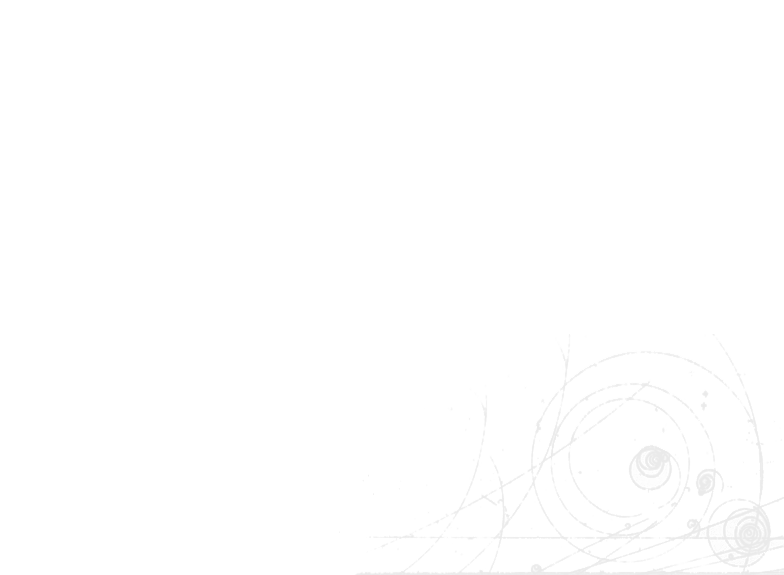
\includegraphics[width=\paperwidth,height=\paperheight]{BG_lower}}}

%% \begin{frame}% [<+->]
%% %% {About me}
%% \frametitle{\centerline{Outline}}

%% \begin{itemize}
%% \setlength\itemsep{10pt}
%% \item<1-> Current status, operating service
%% \item<1-> user guide, howto take part
%% \item<1-> Recent improvements
%% \item<1-> HLT rate
%% \item<1-> Gauss timing
%% \item<1-> throughput
%% \item<1-> Big data tools (+my thoughts on it)
%% \end{itemize}
%% \end{frame}

\begin{frame}% [<+->]
%% {About me}
\frametitle{\centerline{LHCb Performance and Regression framework}}
\begin{itemize}
\setlength\itemsep{10pt}
\item<1-> {\bf LHCbPR} is a framework for systematic monitoring of the LHCb software
\item<1-> Provides performance baseline in {\bf controlled conditions}
\item<1-> Enables to {\bf inspect any changes} due to e.g. MC generators, physics of Geant4, new external libraries, new MRs, DDDB tags, ...
\item<1-> {\bf Compare results} across different compilers and architectures
\item<1-> Not only to monitor resource consumption, but also to {\bf measure the physics~performance}
\item<1-> Cf. nightly tests: larger statistics and more than boolean value
%% \item<1-> {\bf Loosely coupled modules} communicating through simple API's
\end{itemize}
\end{frame}

\begin{frame}[fragile]
\frametitle{\centerline{Infrastructure}}
 \href{https://twiki.cern.ch/twiki/bin/view/LHCb/LHCbPR}{\beamergotobutton{TWiki}}
\begin{columns}
\column{0.9\textwidth}
\begin{itemize}
\footnotesize
\item<1-> Periodic tests started by the {\bf Jenkins} job
 \begin{itemize}
 \item<1-> \href{https://jenkins-lhcb-nightlies.web.cern.ch/job/periodic-tests/job/tests-poll/}{\beamergotobutton{Configuration of Jenkins job}}
 \item<1-> \scriptsize tests triggered when corresponding nightly builds ready (using RabbitMQ)
 \end{itemize}
\end{itemize}
\column{0.1\textwidth}
\visible<1->{
\centering  
\includegraphics[width=0.9\textwidth]{figures/jenkins.png}}
%% \visible<2->{
%% 
\includegraphics[width=0.99\textwidth]{figures/slc6.png}} 
%% \visible<2->{
%% 
\includegraphics[width=0.99\textwidth]{figures/centos7.png}} 
\end{columns}
\begin{itemize}
\footnotesize
\item<2-> Configuration in {\bf XML} files
 \begin{itemize}
\item<2-> \href{https://gitlab.cern.ch/lhcb-core/LHCbNightlyConf/blob/master/test_schedule2.xml}{\beamergotobutton{LHCbNightlyConf}}
\end{itemize}
\item<3-> Machines that tests are currently running on
\begin{itemize}
\scriptsize
\item<3-> \texttt{lblhcbpr1} with CC7 dedicated for timing tests (single executor in Jenkins), label: \texttt{perf-centos7-timing}
\item<3-> \texttt{lblhcbpr4} with CC7 (8 executors), labels: \texttt{perf-centos7, perf}
\item<3-> \texttt{volhcb05} with SLC6 (8 executors), labels: \texttt{perf-slc6, perf}
\item<3-> \texttt{hltperf-quanta01-e52630v4} for HLT throughput test
\item<3-> \texttt{lbhltperf01} for upgrade tests
\end{itemize}

 \end{itemize}

%% 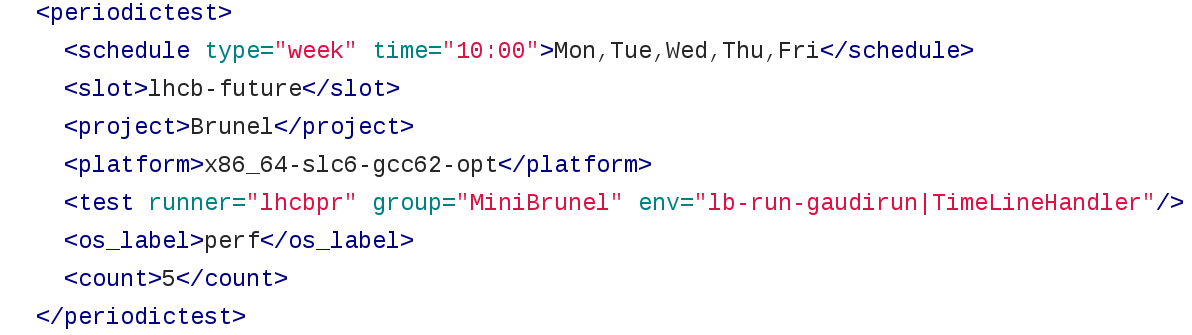
\includegraphics[width=0.99\textwidth]{figures/schedule2.png}} 
\end{frame}

\begin{frame}[fragile]
\frametitle{\centerline{Infrastructure}}
\begin{columns}
\column{0.9\textwidth}
\begin{itemize}
\footnotesize
\item<1-> Results of the tests {\bf parsed by the specific handlers}
\begin{itemize}
\scriptsize
\item<1-> \href{https://gitlab.cern.ch/lhcb-core/LHCbPR2HD}{\beamergotobutton{LHCbPR2HD}}
\item<1-> to save relevant metrics (int, float, string, ROOT, JSON)
\end{itemize}
\item<2-> Zip file sent to the database through {\bf Dirac Storage Element} \verb|/lhcb/prdata/zips|
\begin{itemize}
\scriptsize
\item<2-> \href{https://gitlab.cern.ch/lhcb-core/LHCbPR2BE}{\beamergotobutton{LHCbPR2BE}}
\end{itemize}
\end{itemize}
\column{0.1\textwidth}
\visible<1->{

\includegraphics[width=0.99\textwidth]{figures/python.png}} 
\visible<2->{
\centering 
\includegraphics[width=0.99\textwidth]{figures/mysql.png}}
\visible<2->{
\centering 
\includegraphics[width=0.99\textwidth]{figures/dirac.png} } \\
\end{columns}

\begin{columns}
\column{0.5\textwidth}
\begin{itemize}
\footnotesize
\item<4-> {\bf Web front--end} \href{http://lblhcbpr.cern.ch/}{\beamergotobutton{lblhcbpr.cern.ch}}
\begin{itemize}
\scriptsize
\item<4-> \href{https://gitlab.cern.ch/lhcb-core/LHCbPR2FE}{\beamergotobutton{LHCbPR2FE}}
\item<4-> generic ROOT files viewer
\item<4-> trend analysis
\item<4-> custom modules
\end{itemize}
\item<5-> Flexibility to push the results as HTML to EOS (at the level of LHCbPR2HD)
\begin{itemize}
\scriptsize
\item<5-> HLT rate and throughput tests
\item<5-> upgrade benchmarking
\end{itemize}
\end{itemize}
\column{0.5\textwidth}
\begin{center}
\visible<4->{
{\centering 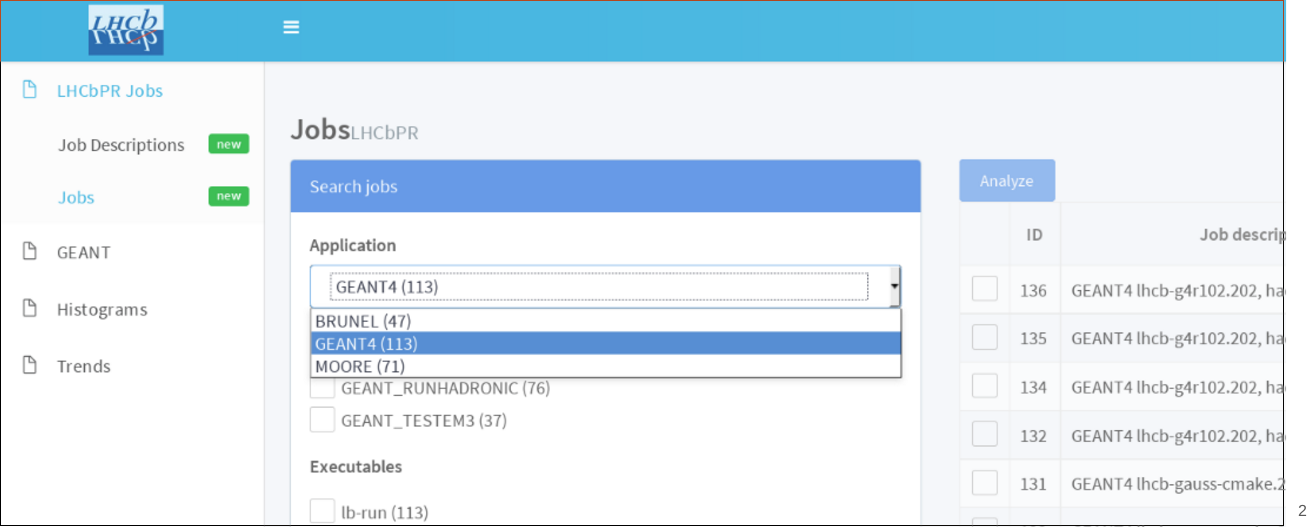
\includegraphics[width=0.87\textwidth]{figures/frontend.png} }}
\end{center}
\end{columns}

\end{frame}

\begin{frame}% [<+->]
%% {About me}
\frametitle{\centerline{Some statistics as of today}}
\begin{itemize}
\footnotesize
\setlength\itemsep{10pt}
\item<1-> 5 applications
\begin{itemize}
\scriptsize
\item<1-> Brunel
\item<1-> Gauss
\item<1-> Geant4
\item<1-> Moore
\item<1-> MooreOnline
\end{itemize}
\item<1-> 67 option files
\item<1-> 128 tests (running on several slots and platforms)
\item<1-> $\sim$50 tests daily
\item<1-> $\sim$20 tests dedicated for timing (thus running only on \texttt{lblhcbpr1} machine)
\item<1-> Single tests run from several minutes up to 10 hours
%% \item<1-> In practice, timing machine busy for significant amount of time, but the others are relatively free
\end{itemize}
\end{frame}

\begin{frame}[fragile]
\frametitle{\centerline{How to take part}}
\begin{itemize}
\footnotesize
\item<1-> Prepare the {\bf options file} for the test and commit to e.g. PRConfig
\item<2-> Specify the {\bf command} to run
\begin{itemize}
\scriptsize
\item<2-> see whether it's already defined: \href{https://lblhcbpr.cern.ch/api/executables/}{\beamergotobutton{lblhcbpr.cern.ch/api/executables}}, if not, we'll add it
\tiny
            \begin{verbatim}
 "name": "lb-run-gaudirun",
 "content": "lb-run -c {platform} --user-area={build} {app_name}/{app_version} 
            gaudirun.py {options}"
            \end{verbatim}
            \begin{verbatim}
 "name": "lb-run-callgrind",
 "content": "( lb-run -c {platform} --user-area={build} {app_name}/{app_version} gaudirun.py
               --printsequence {options} ; lb-run -c {platform} --user-area={build}
               {app_name}/{app_version} valgrind --tool=callgrind --dump-instr=yes
               --instr-atstart=no --cache-sim=yes --branch-sim=yes python
               $(lb-run -c {platform} --user-area={build} {app_name}/{app_version}
                        which gaudirun.py) {options} )"
            \end{verbatim}
            \begin{verbatim}
 "name": "perf-lb-run-gaudirun",
 "content": "( perf record --call-graph=lbr -o perf.log lb-run -c {platform} 
            --user-area={build} {app_name}/{app_version} gaudirun.py {options} ; 
            perf report -i perf.log > perf.lbr.txt )"
            \end{verbatim}

\end{itemize}
\item<3-> Create the {\bf handler} to parse the output
\begin{itemize}
\scriptsize
\item<3-> many handlers already there, e.g. to parse \texttt{TimingAuditor}, output of \texttt{perf}, etc.
\item<3-> see README on: \href{https://gitlab.cern.ch/lhcb-core/LHCbPR2HD/blob/master/README.md}{\beamergotobutton{LHCbPR2HD}}
\end{itemize}
\end{itemize}
\end{frame}

\begin{frame}[fragile]
\frametitle{\centerline{How to take part}}
\begin{itemize}
\footnotesize
\item<1-> {\bf Schedule} your test in \href{https://gitlab.cern.ch/lhcb-core/LHCbNightlyConf/blob/master/test_schedule2.xml}{\beamergotobutton{LHCbNightlyConf}}
\end{itemize}

\begin{tikzpicture}%[show background grid] %% Use grid for positioning, then turn off
\visible<2->{

		\node [inner sep=0pt,above right] 
			{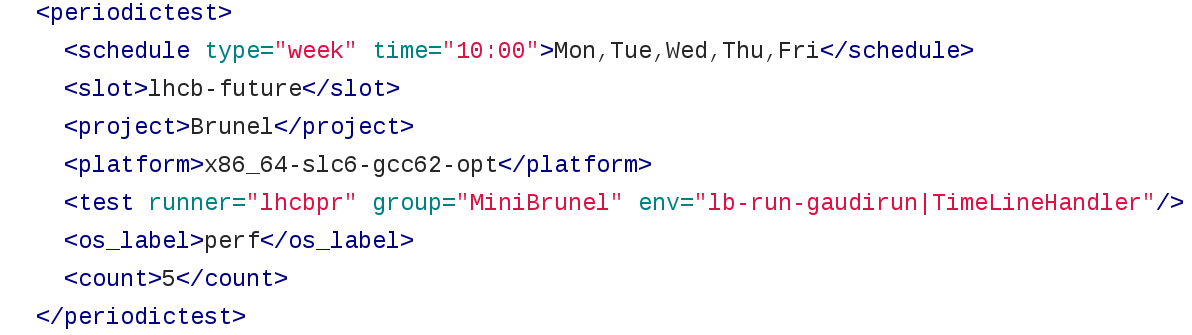
\includegraphics[width=0.99\textwidth]{figures/schedule2.png}};
}
		% \node[right] at (.5,8) {\Comment{\ECFAugie(Left of this ruled out)}};
		%% \node[right]  at (0,0) {\footnotesize\textcolor{Comment}{1104.3572}};
\visible<3->{
		\node[right] (mag) at (7,3.6) {\scriptsize\textcolor{magenta}{schedule weekly or monthly}};
}
\visible<4->{
		\node[right] (cya) at (6.8,2.7) {\scriptsize\textcolor{cyan}{description of options \url{lblhcbpr.cern.ch/api/options}}};
}
\visible<5->{
		\node[right] (blu) at (9,2.1) {\scriptsize\textcolor{blue}{executable and handler}};
}
\visible<6->{
		\node[right] (gre) at (6,1) {\scriptsize\textcolor{FlipGreen}{machine label}};
}
		%% \node[right] (mag) at (7.5,1.5) {\footnotesize\textcolor{magenta}{stop co-annihilations}};
		 \node (magdot) at (3.3,3.3) {};
		 \node (cyadot) at (5.5,1.5) {};
		 \node (bludot) at (8.1,1.6) {};
		 \node (gredot) at (2.5,1.1) {};
		%% \node (magdot) at (3,1.3) {};
\visible<3->{
		 \path[->, color=magenta, line width=1] (mag) edge [out = 160, in = 45] (magdot);
}
\visible<4->{
		 \path[->, color=cyan, line width=1] (cya) edge [out = 170, in = 45] (cyadot);
}
\visible<5->{
		 \path[->, color=blue, line width=1] (blu) edge [out = 180, in = 45] (bludot);
}
\visible<6->{
		 \path[->, color=FlipGreen, line width=1] (gre) edge [out = 170, in = 45] (gredot);
}
		%% \path[->, color=magenta, line width=1.5] (mag) edge [out = 185, in = 15] (magdot);
\end{tikzpicture}
\end{frame}

\begin{frame}[fragile]
\frametitle{\centerline{How to use LHCbPR}}
\begin{itemize}
\footnotesize
\item<1-> Tests will automatically start on a day given by schedule (if the nightly build is ok)
\item<1-> You will see {\bf \textcolor{blue}{PR}} link in the nightlies dashboard, close to the project name in the given slot 
\item<2-> Watch the tests being executed in \href{https://lbnightlies.cern.ch/periodic/}{\beamergotobutton{dashboard}}
\begin{itemize}
\scriptsize
\item<2-> colour code: \textcolor{blue}{running tests}, \textcolor{green}{successful tests}, \textcolor{red}{failed tests}, \textcolor{orange}{tests which have been executed with success, but the handler failed} 
\item<2-> URL to log files of the test, handler and output of the Jenkins job
\end{itemize}
\item<3-> You can launch the test yourself from the dashboard
\begin{itemize}
\scriptsize
\item<3-> e.g. to the test the handler
\item<3-> click on {\bf Start new periodic test} button (available after login)
\end{itemize}
\item<4-> To see the results of the test, by default you can use generic {\bf trend analysis} and {\bf ROOT file viewer} on \url{lblhcbpr.cern.ch}
\item<5-> (Optionally) create custom {\bf analysis module} \href{https://gitlab.cern.ch/lhcb-core/LHCbPR2FE/blob/master/documentation/modules-guide.md}{\beamergotobutton{LHCbPR2FE}}
\begin{itemize}
\scriptsize
\item<5-> or re-use existing one ...
\end{itemize}
\end{itemize}
\end{frame}

\begin{frame}[fragile]
\frametitle{\centerline{Trend module with predefined parameters}}
\scriptsize
Plot last 10 measurements for a given algorithm
\begin{tikzpicture}%[show background grid] %% Use grid for positioning, then turn off
\visible<1>{
		\node [inner sep=0pt,above right] 
			{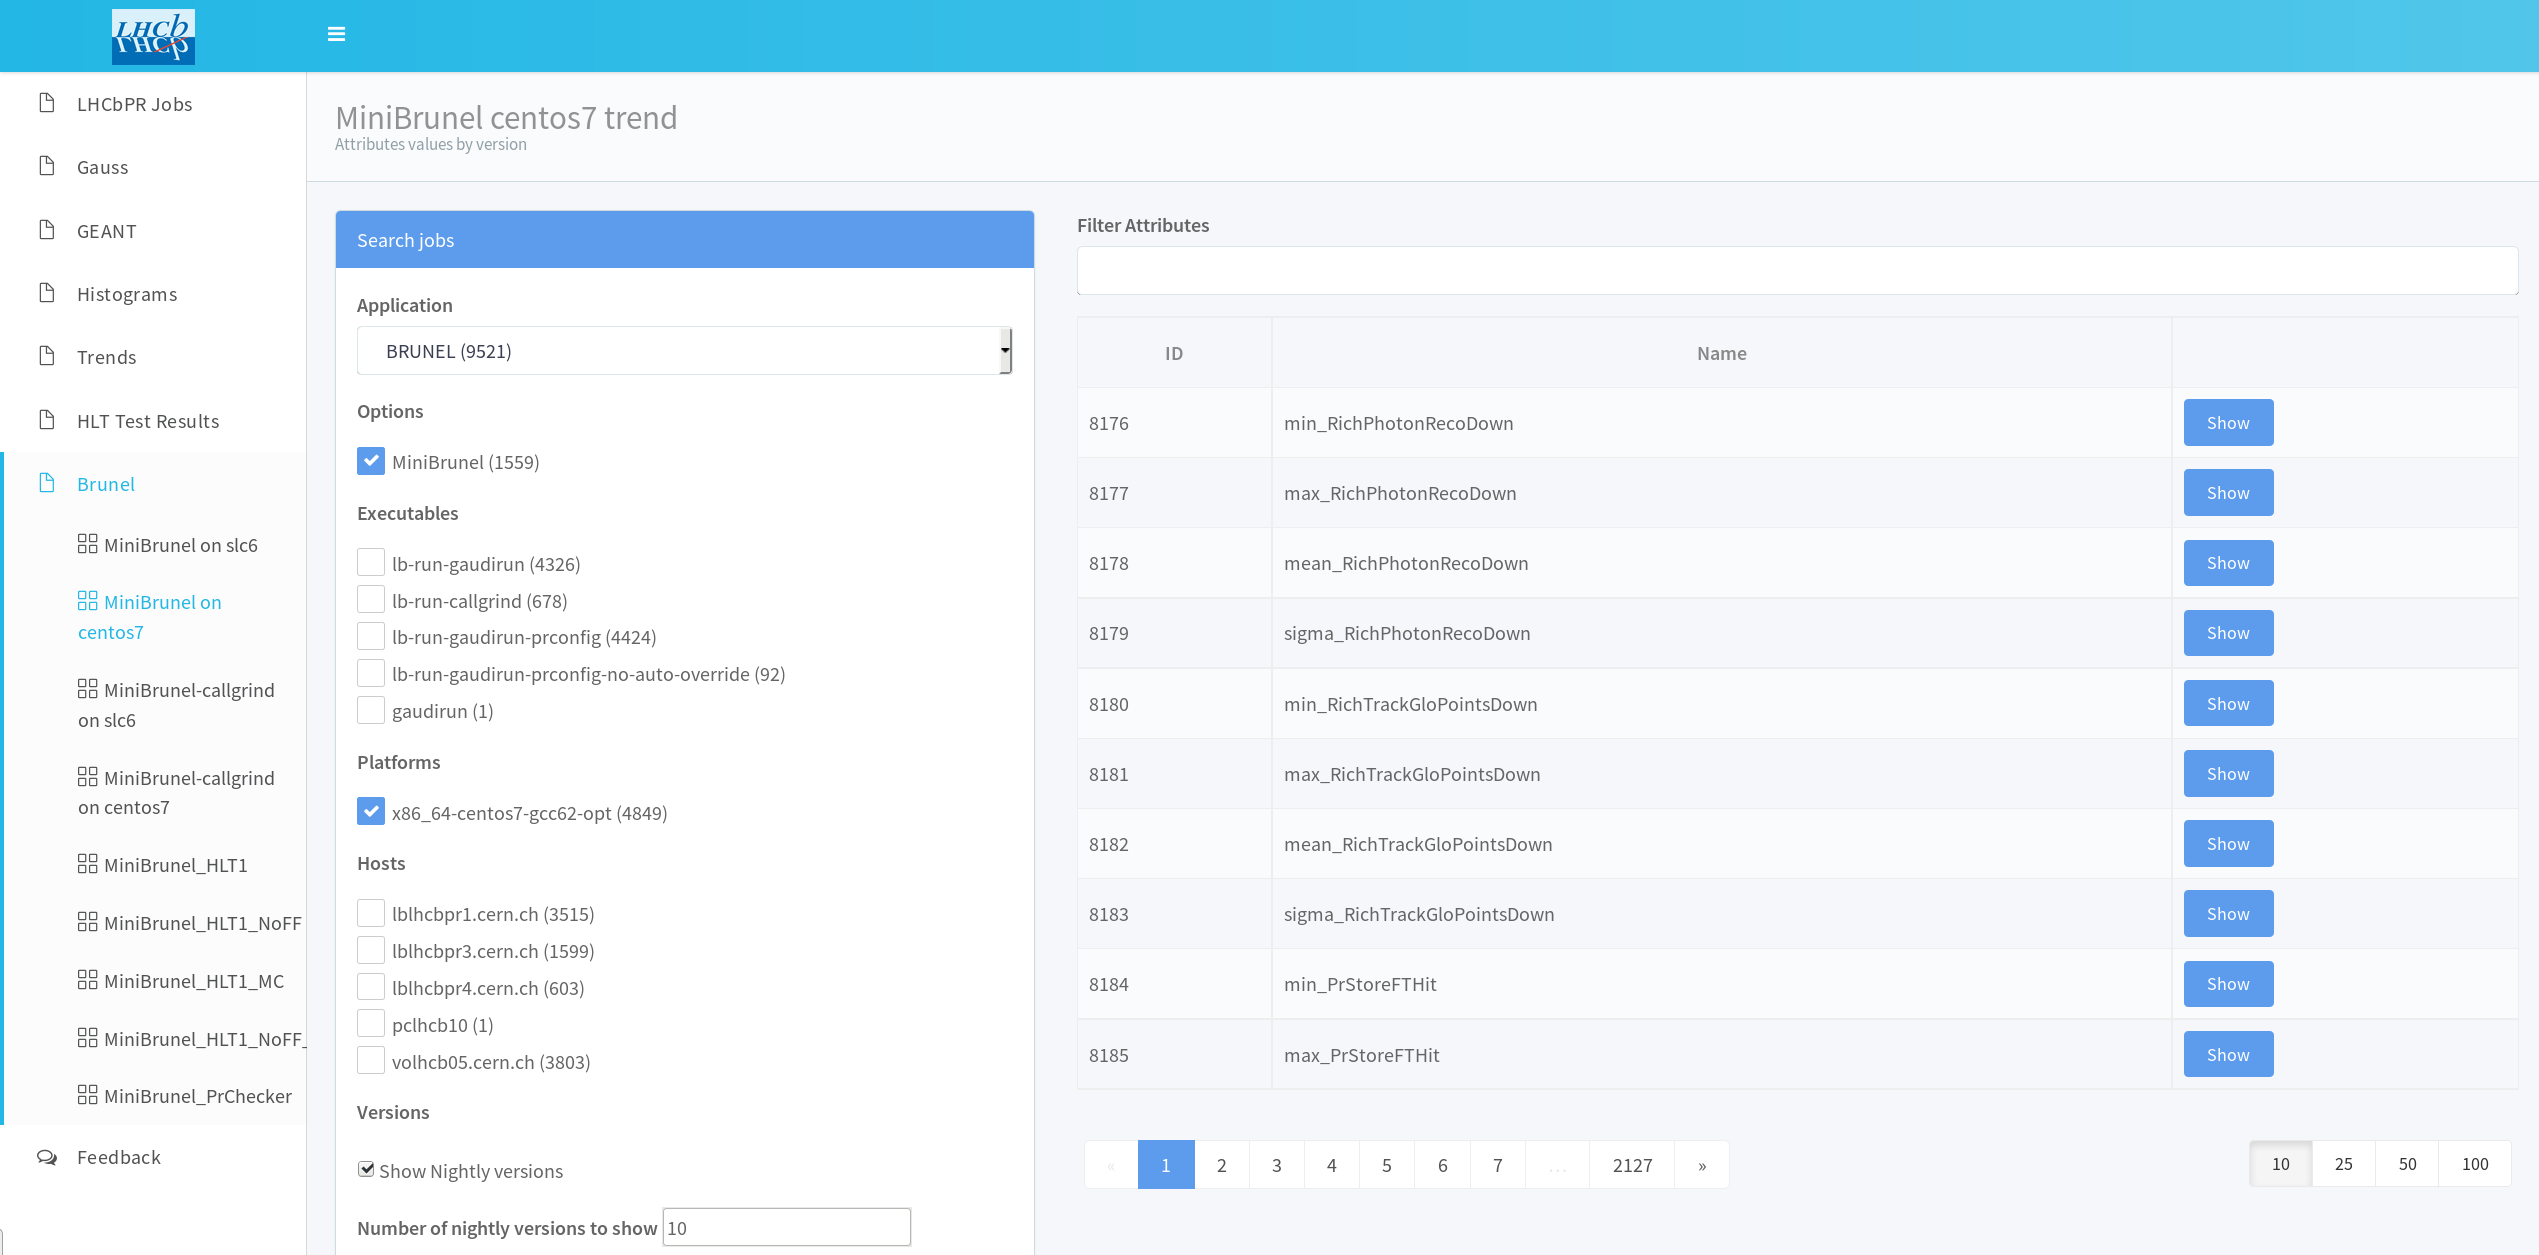
\includegraphics[width=0.99\textwidth]{figures/pred.png}};
}
\end{tikzpicture}
\end{frame}

\begin{frame}[fragile]
\frametitle{\centerline{Using trend analysis}}
\scriptsize
Plot the time spent by EVENT LOOP in Brunel test as a function of the software version
 
\begin{tikzpicture}%[show background grid] %% Use grid for positioning, then turn off
\visible<1-3>{
		\node [inner sep=0pt,above right] 
			{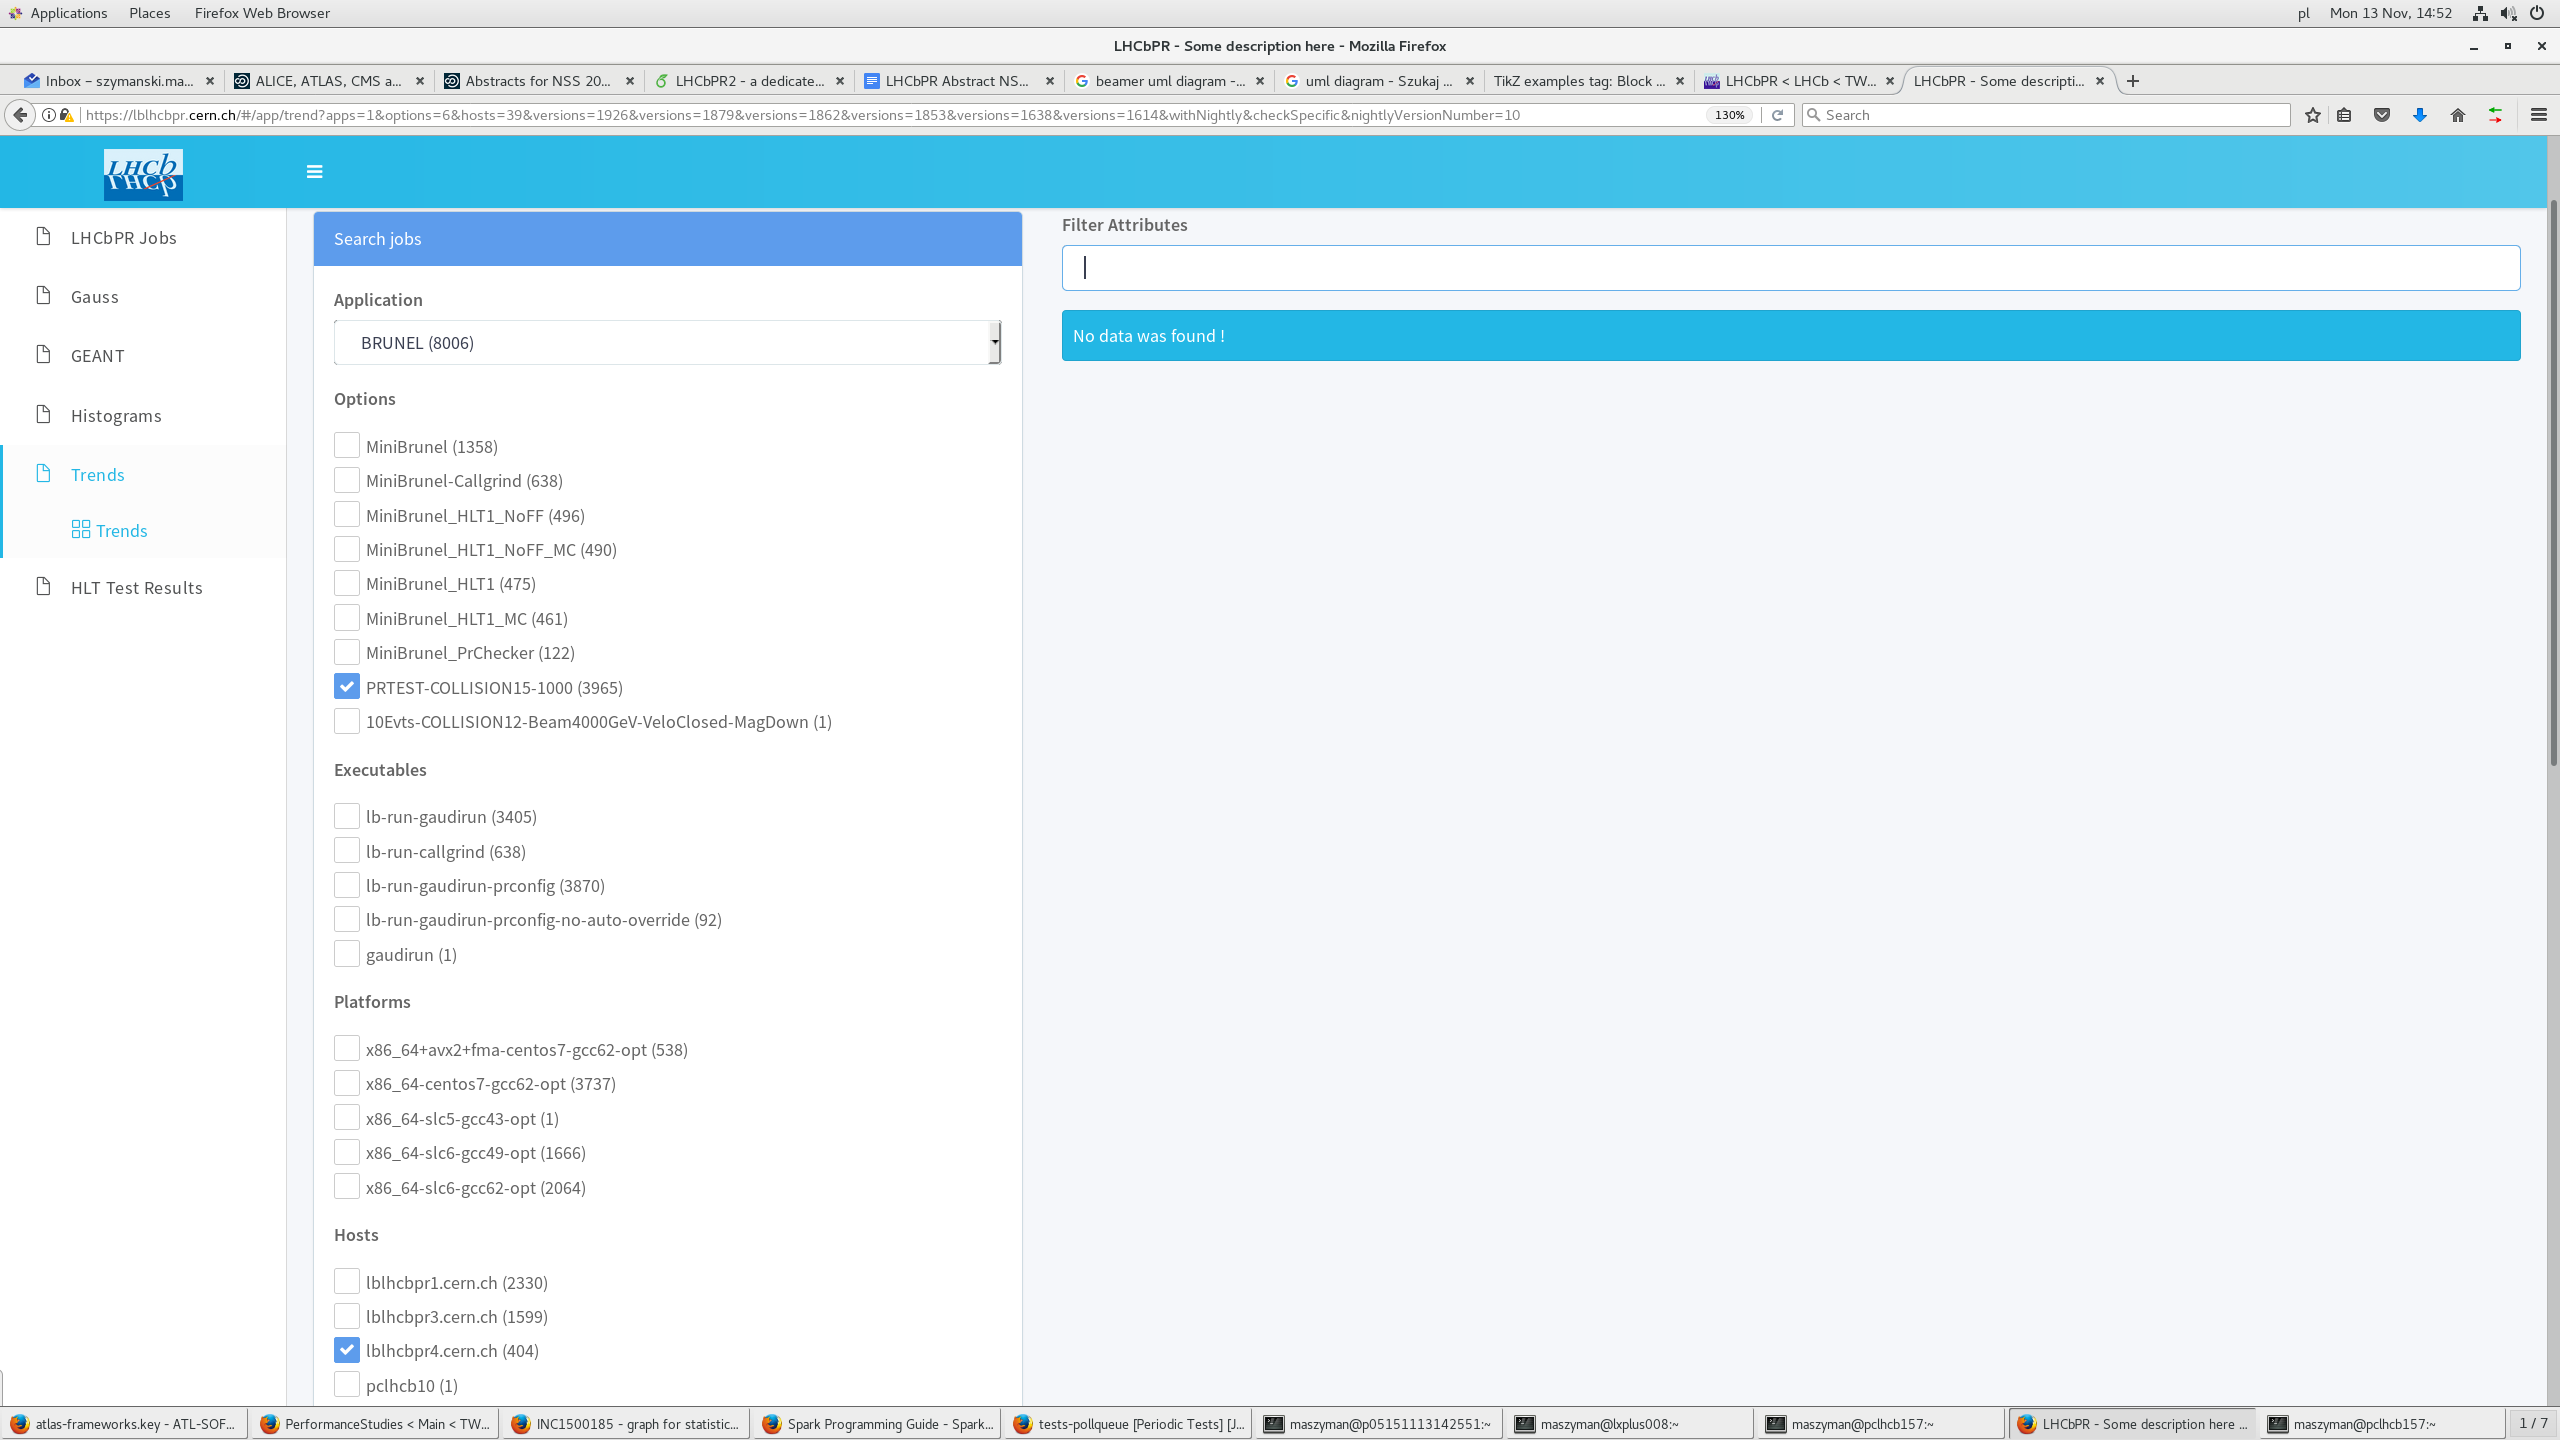
\includegraphics[width=0.99\textwidth]{figures/trend0.png}};
}
\visible<4>{
		\node [inner sep=0pt,above right] 
			{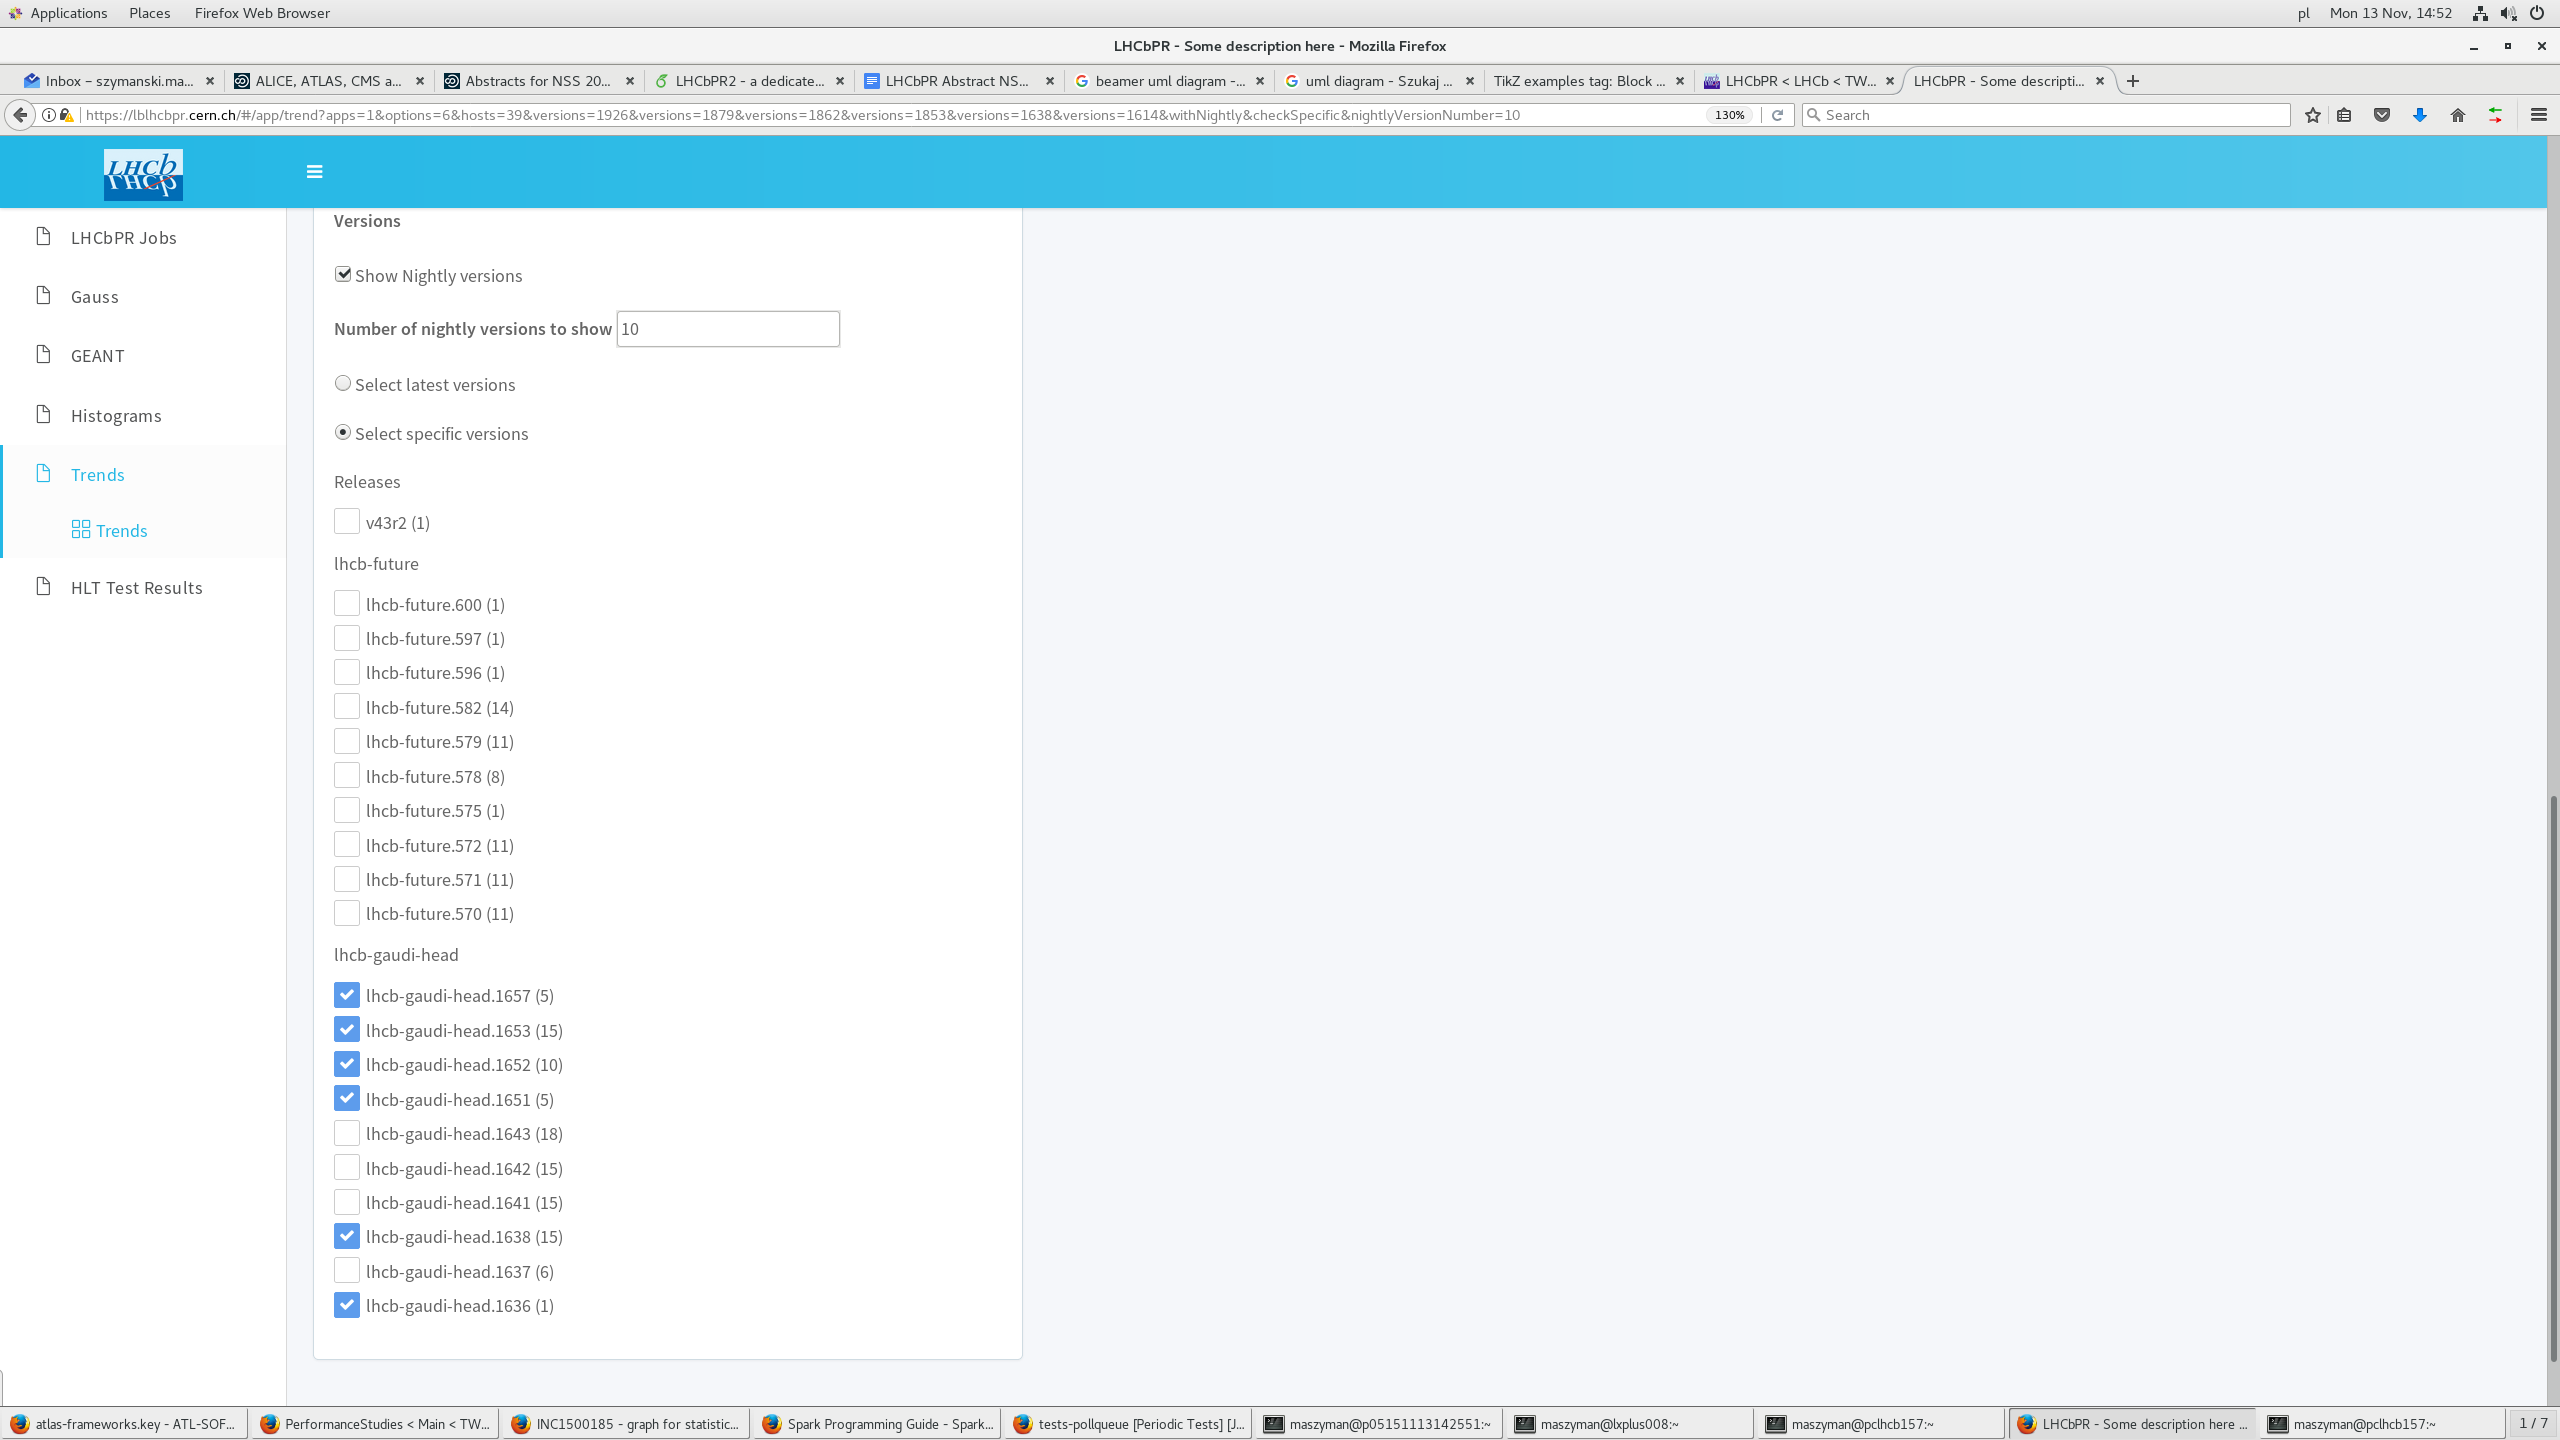
\includegraphics[width=0.99\textwidth]{figures/trend1.png}};
}
\visible<5>{
		\node [inner sep=0pt,above right] 
			{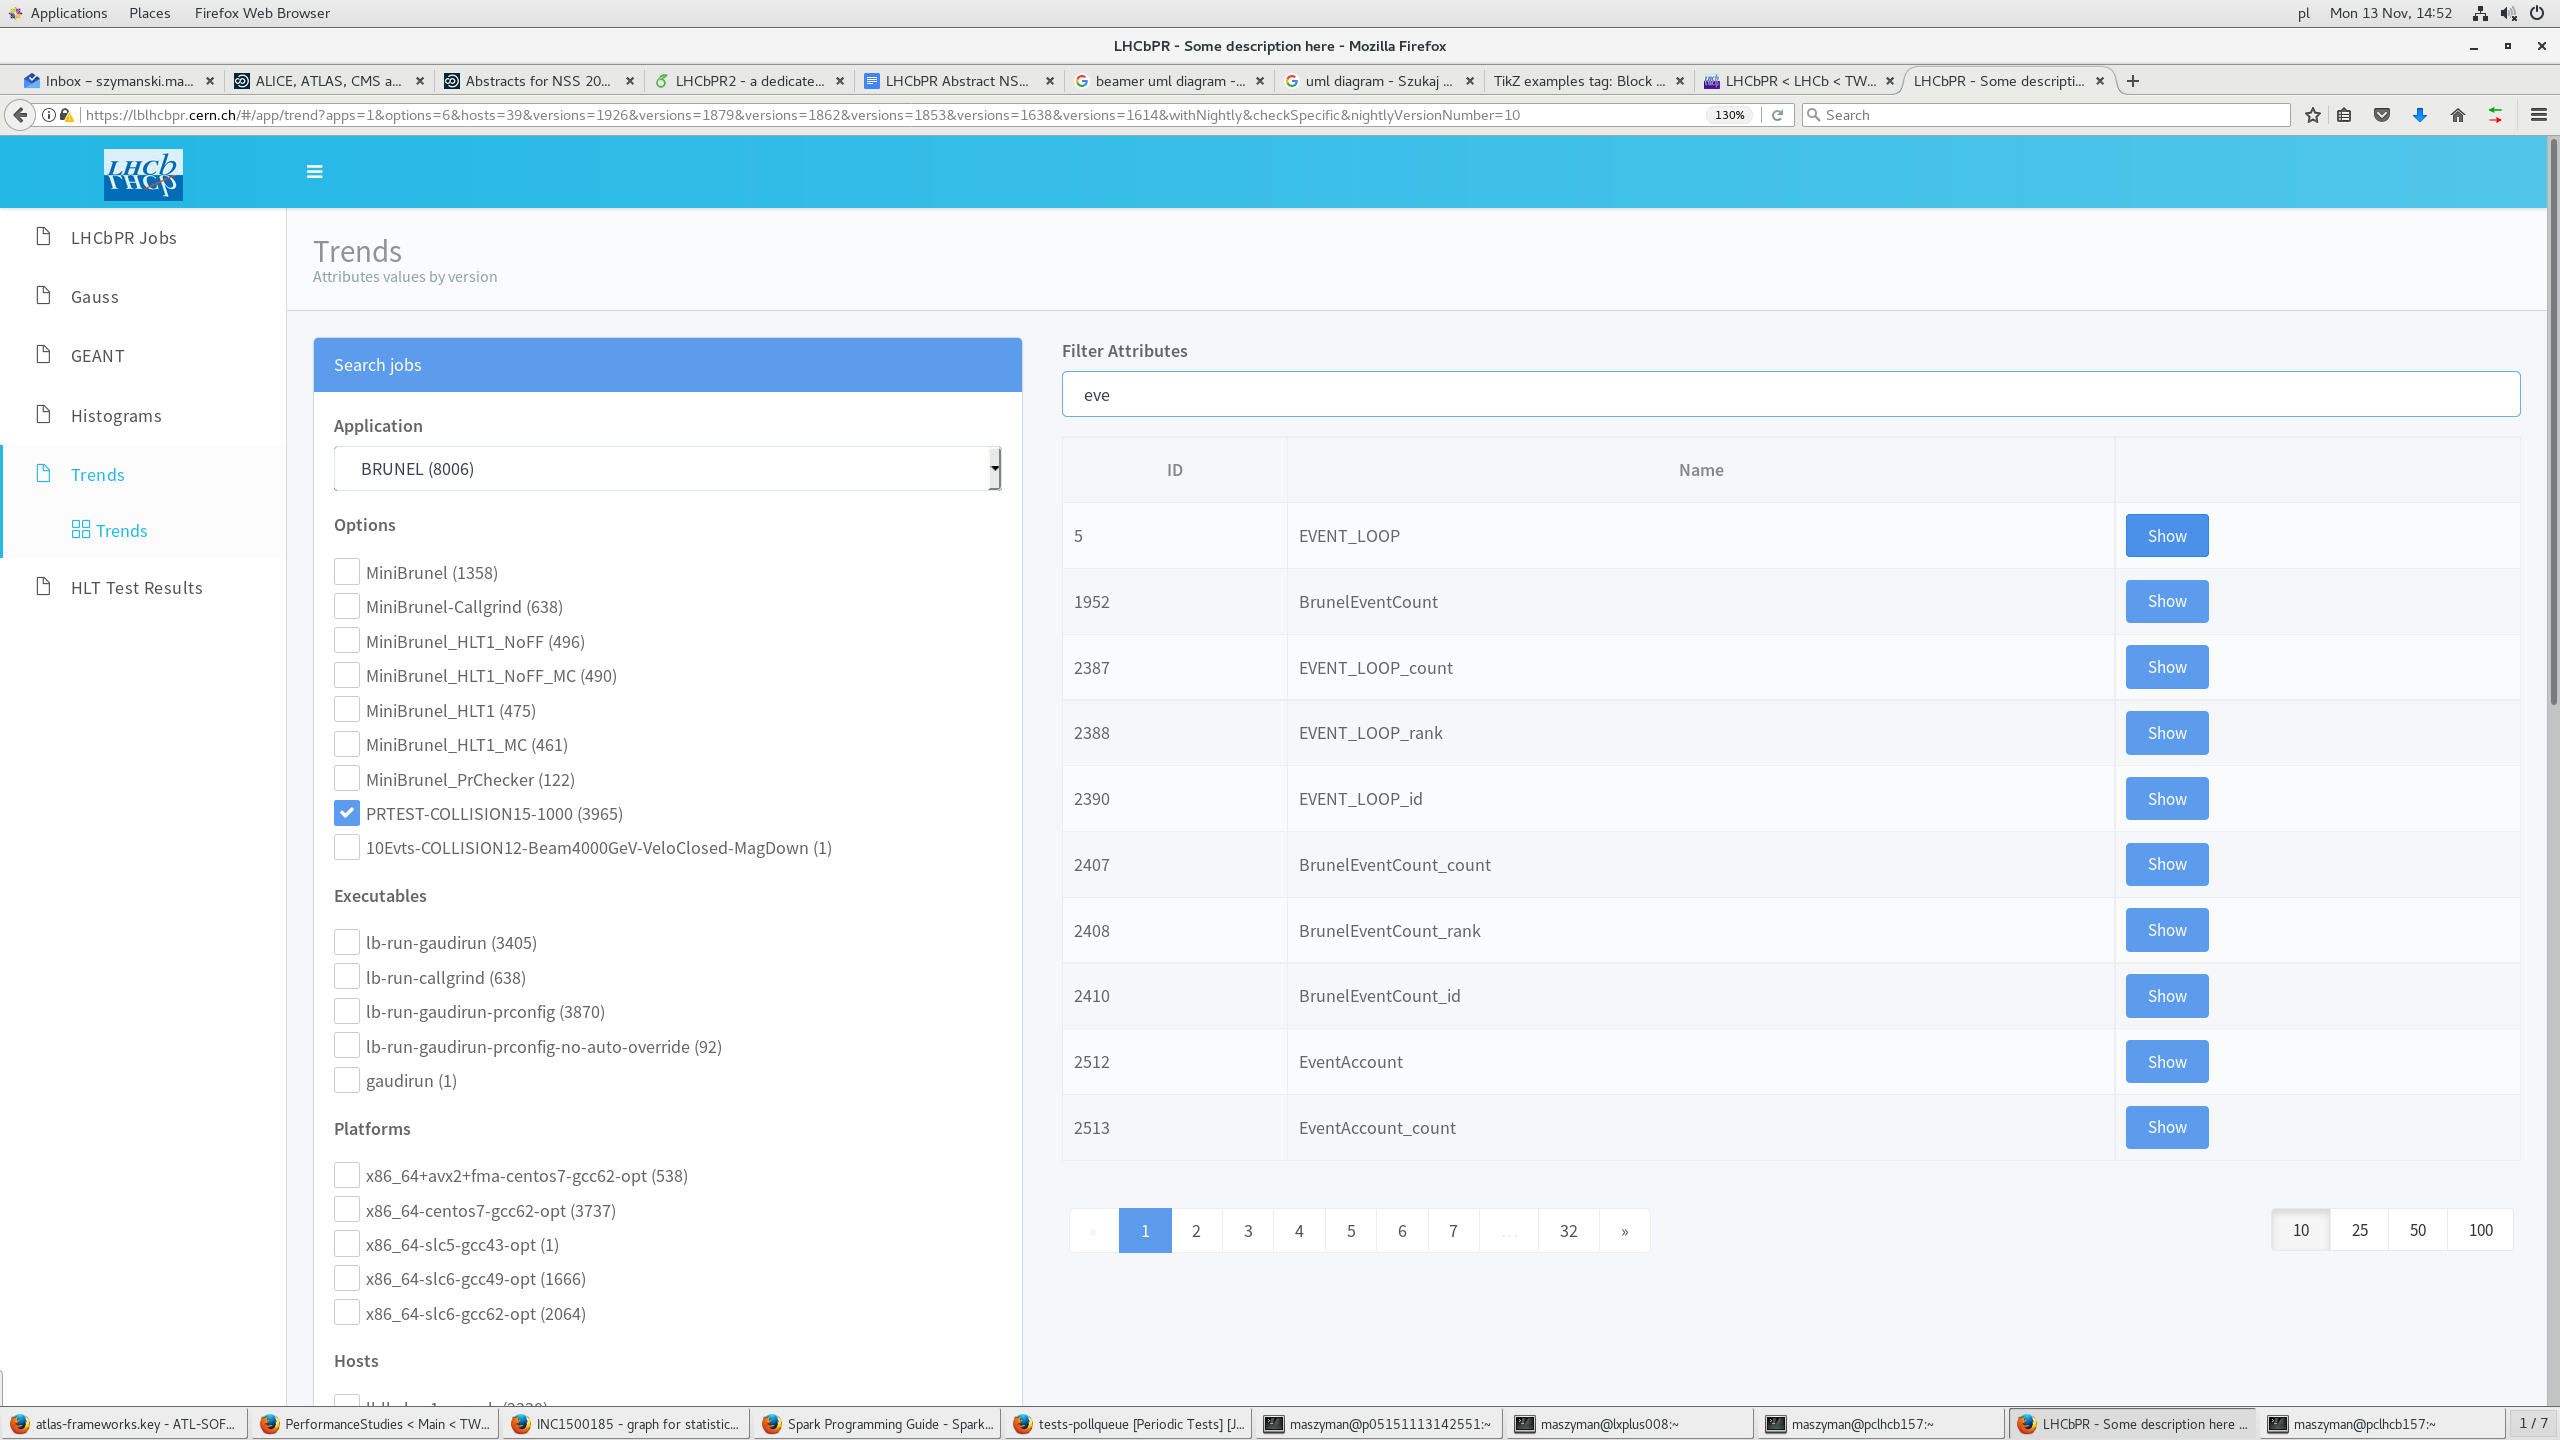
\includegraphics[width=0.99\textwidth]{figures/trend2.png}};
}
\visible<6>{
		\node [inner sep=0pt,above right] 
			{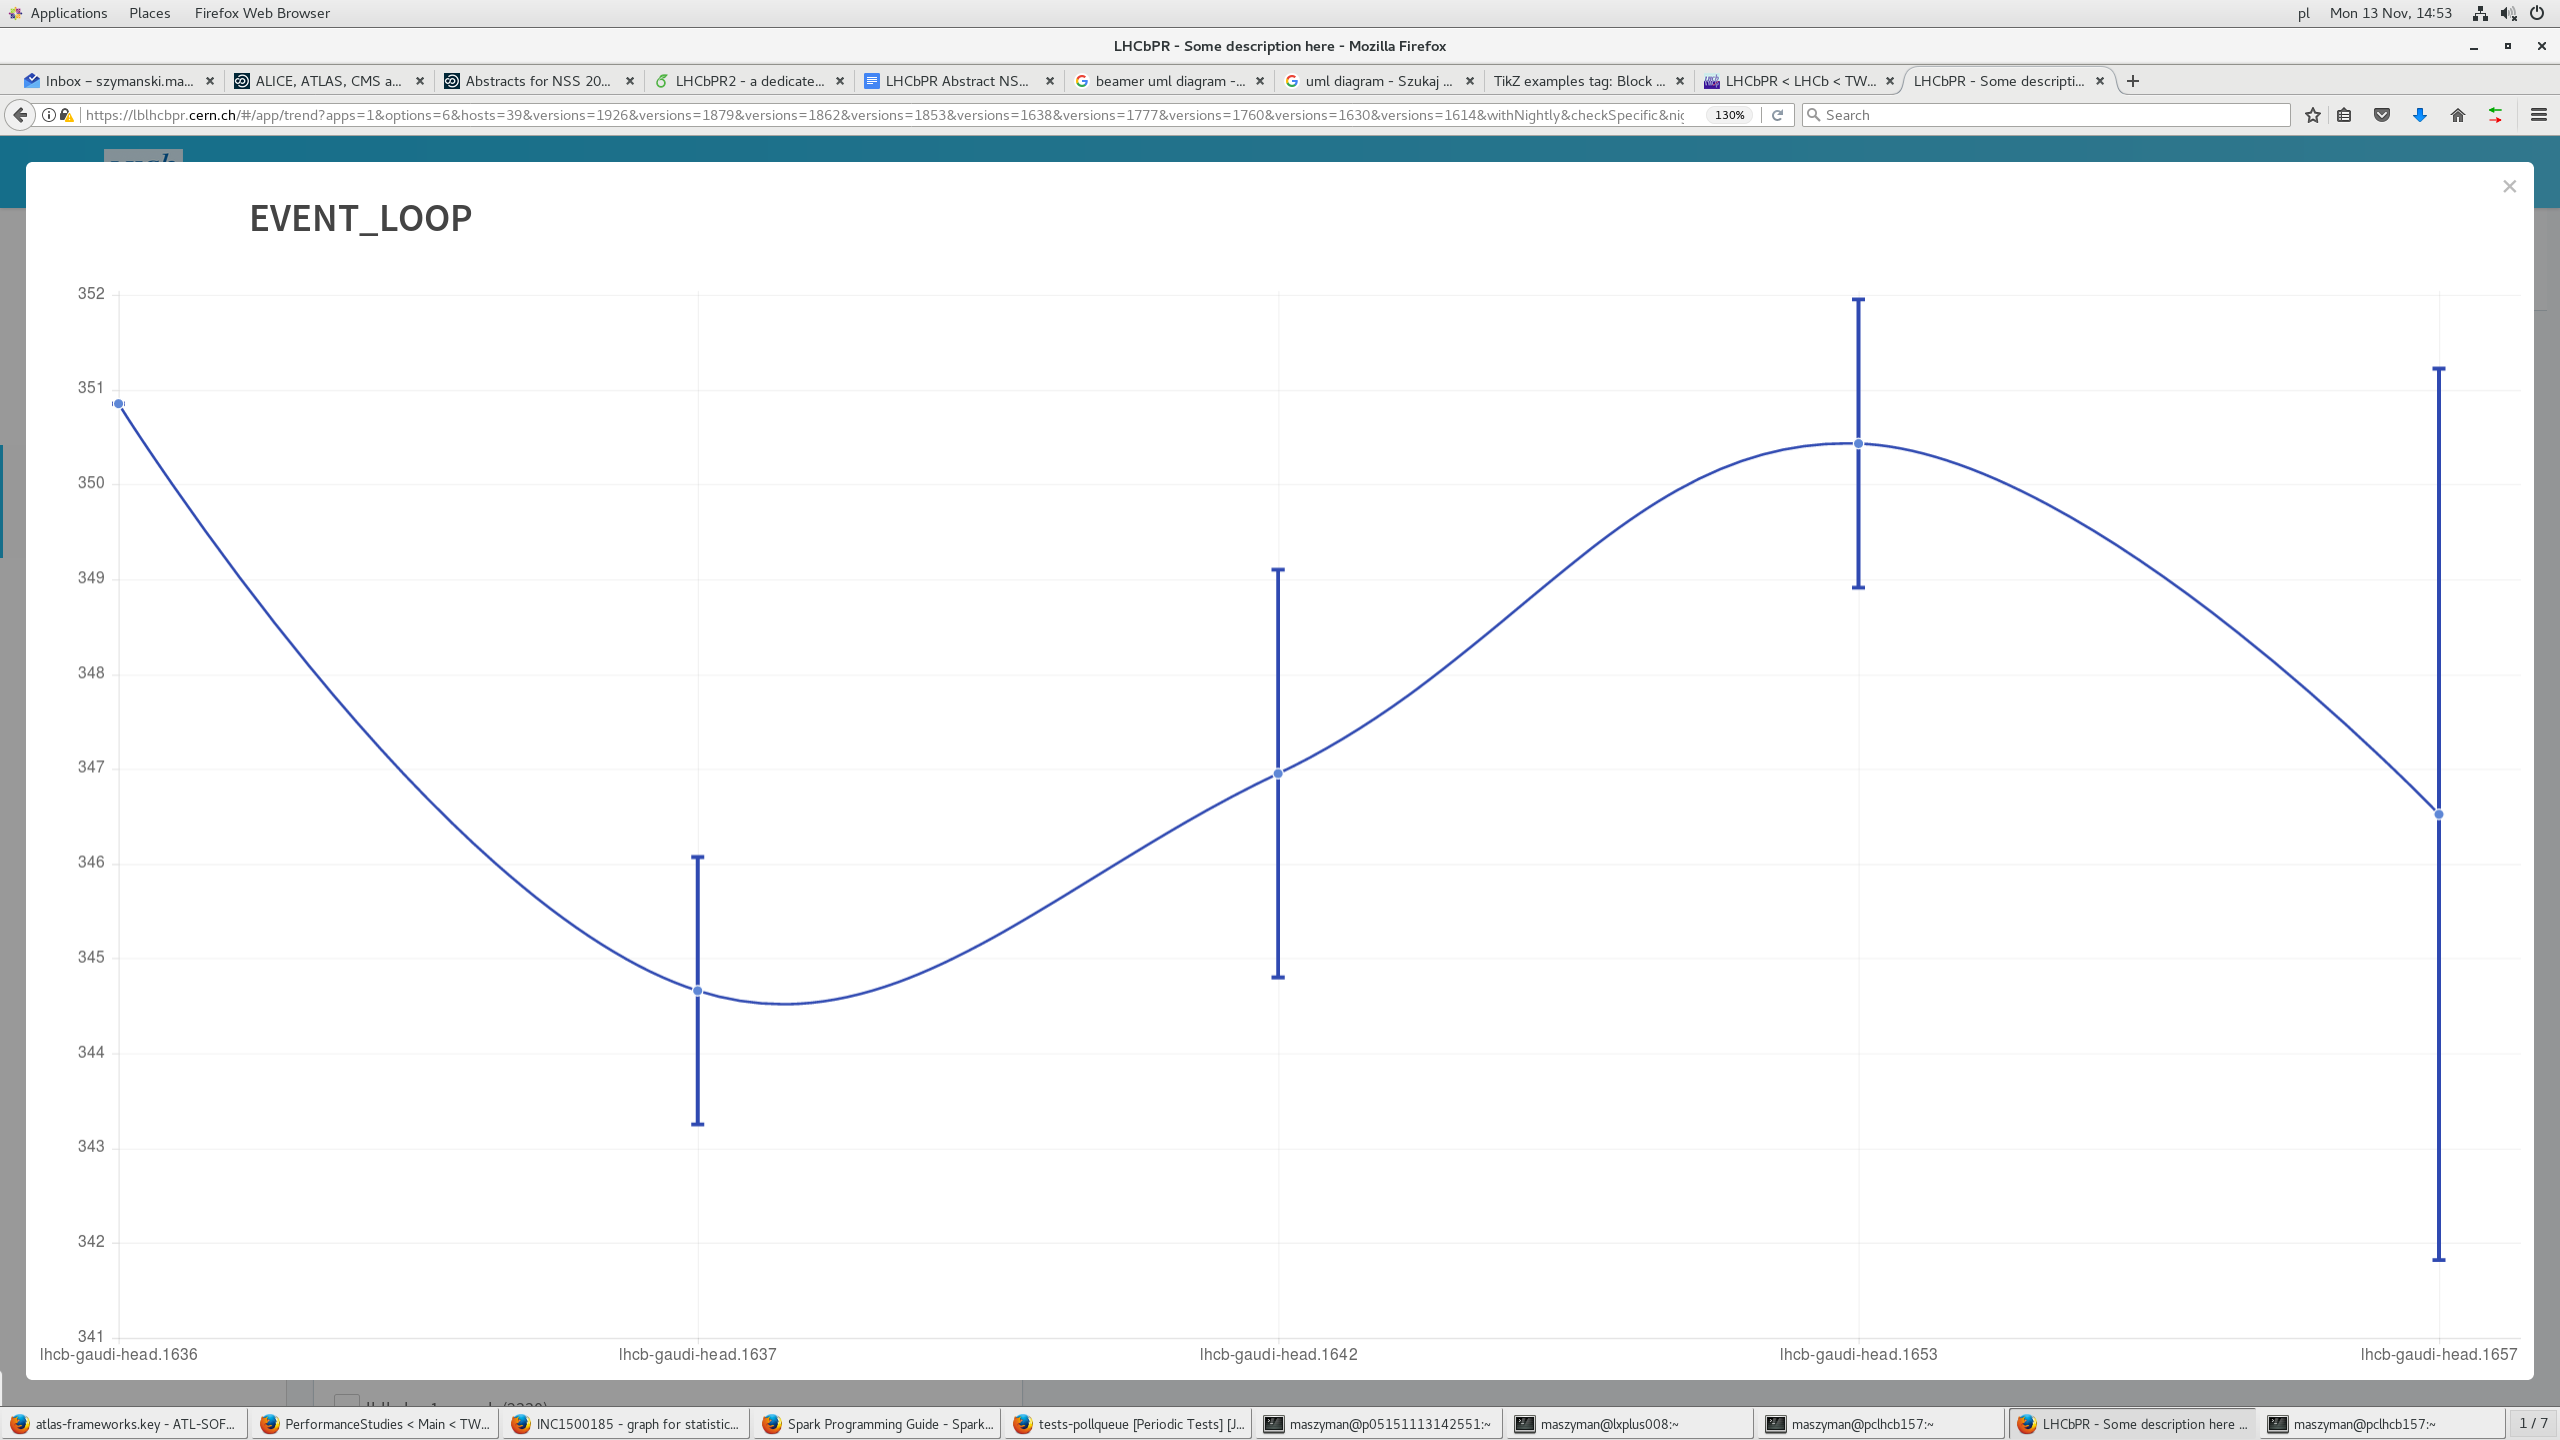
\includegraphics[width=0.99\textwidth]{figures/trend3.png}};
}
\visible<1>{
		\node[right] (blu1) at (6,3) {\scriptsize\textcolor{blue}{go to {\it Trends/Trends} tab}};
}
\visible<2>{
		\node[right] (blu2) at (6,3) {\scriptsize\textcolor{blue}{select Brunel from the list of applications}};
}
\visible<3>{
		\node[right] (blu3) at (6,3) {\scriptsize\textcolor{blue}{select the option, platform and host you are interested in}};
}
\visible<4>{
		\node[right] (blu4) at (6,3) {\scriptsize\textcolor{blue}{choose versions}};
}
\visible<5>{
		\node[right] (blu5) at (8,6) {\scriptsize\textcolor{blue}{type the name of the algorithm}};
}
		 \node (bludot1) at (0.8,5) {};
		 \node (bludot2) at (2.8,6) {};
		 \node (bludot3) at (3.2,4.1) {};
		 \node (bludot4) at (3.2,6.2) {};
		 \node (bludot5) at (6.2,5.6) {};
		 \node (cyadot) at (5.5,1.5) {};
		 \node (bludot) at (8.1,1.6) {};
		 \node (gredot) at (2.5,1.1) {};
\visible<1>{
		 \path[->, color=blue, line width=1] (blu1) edge [out = 160, in = 45] (bludot1);
}
\visible<2>{
		 \path[->, color=blue, line width=1] (blu2) edge [out = 160, in = 45] (bludot2);
}
\visible<3>{
		 \path[->, color=blue, line width=1] (blu3) edge [out = 160, in = 45] (bludot3);
}
\visible<4>{
		 \path[->, color=blue, line width=1] (blu4) edge [out = 160, in = 45] (bludot4);
}
\visible<5>{
		 \path[->, color=blue, line width=1] (blu5) edge [out = 160, in = 45] (bludot5);
}
\end{tikzpicture}
\end{frame}

\begin{frame}
\frametitle{\centerline{Event loop timing in Gauss vs. SW version}}
%% \hfill \textcolor{red}{\tiny see also talk later today in Simulation session}
%% \begin{itemize}
%% \scriptsize
%% \item<1-> \texttt{\$PRCONFIGOPTS/Gauss/PRTEST-2016-SIM-P8-10000000-100evts.py}
%% \item<1-> inclusive b events
%% \item<1-> pp @ 13 TeV
%% \item<1-> 100 events per single test run
%% \item<1-> runs 5 times for statistics
%% \end{itemize}
\begin{center}
%% \visible<1->{
%% 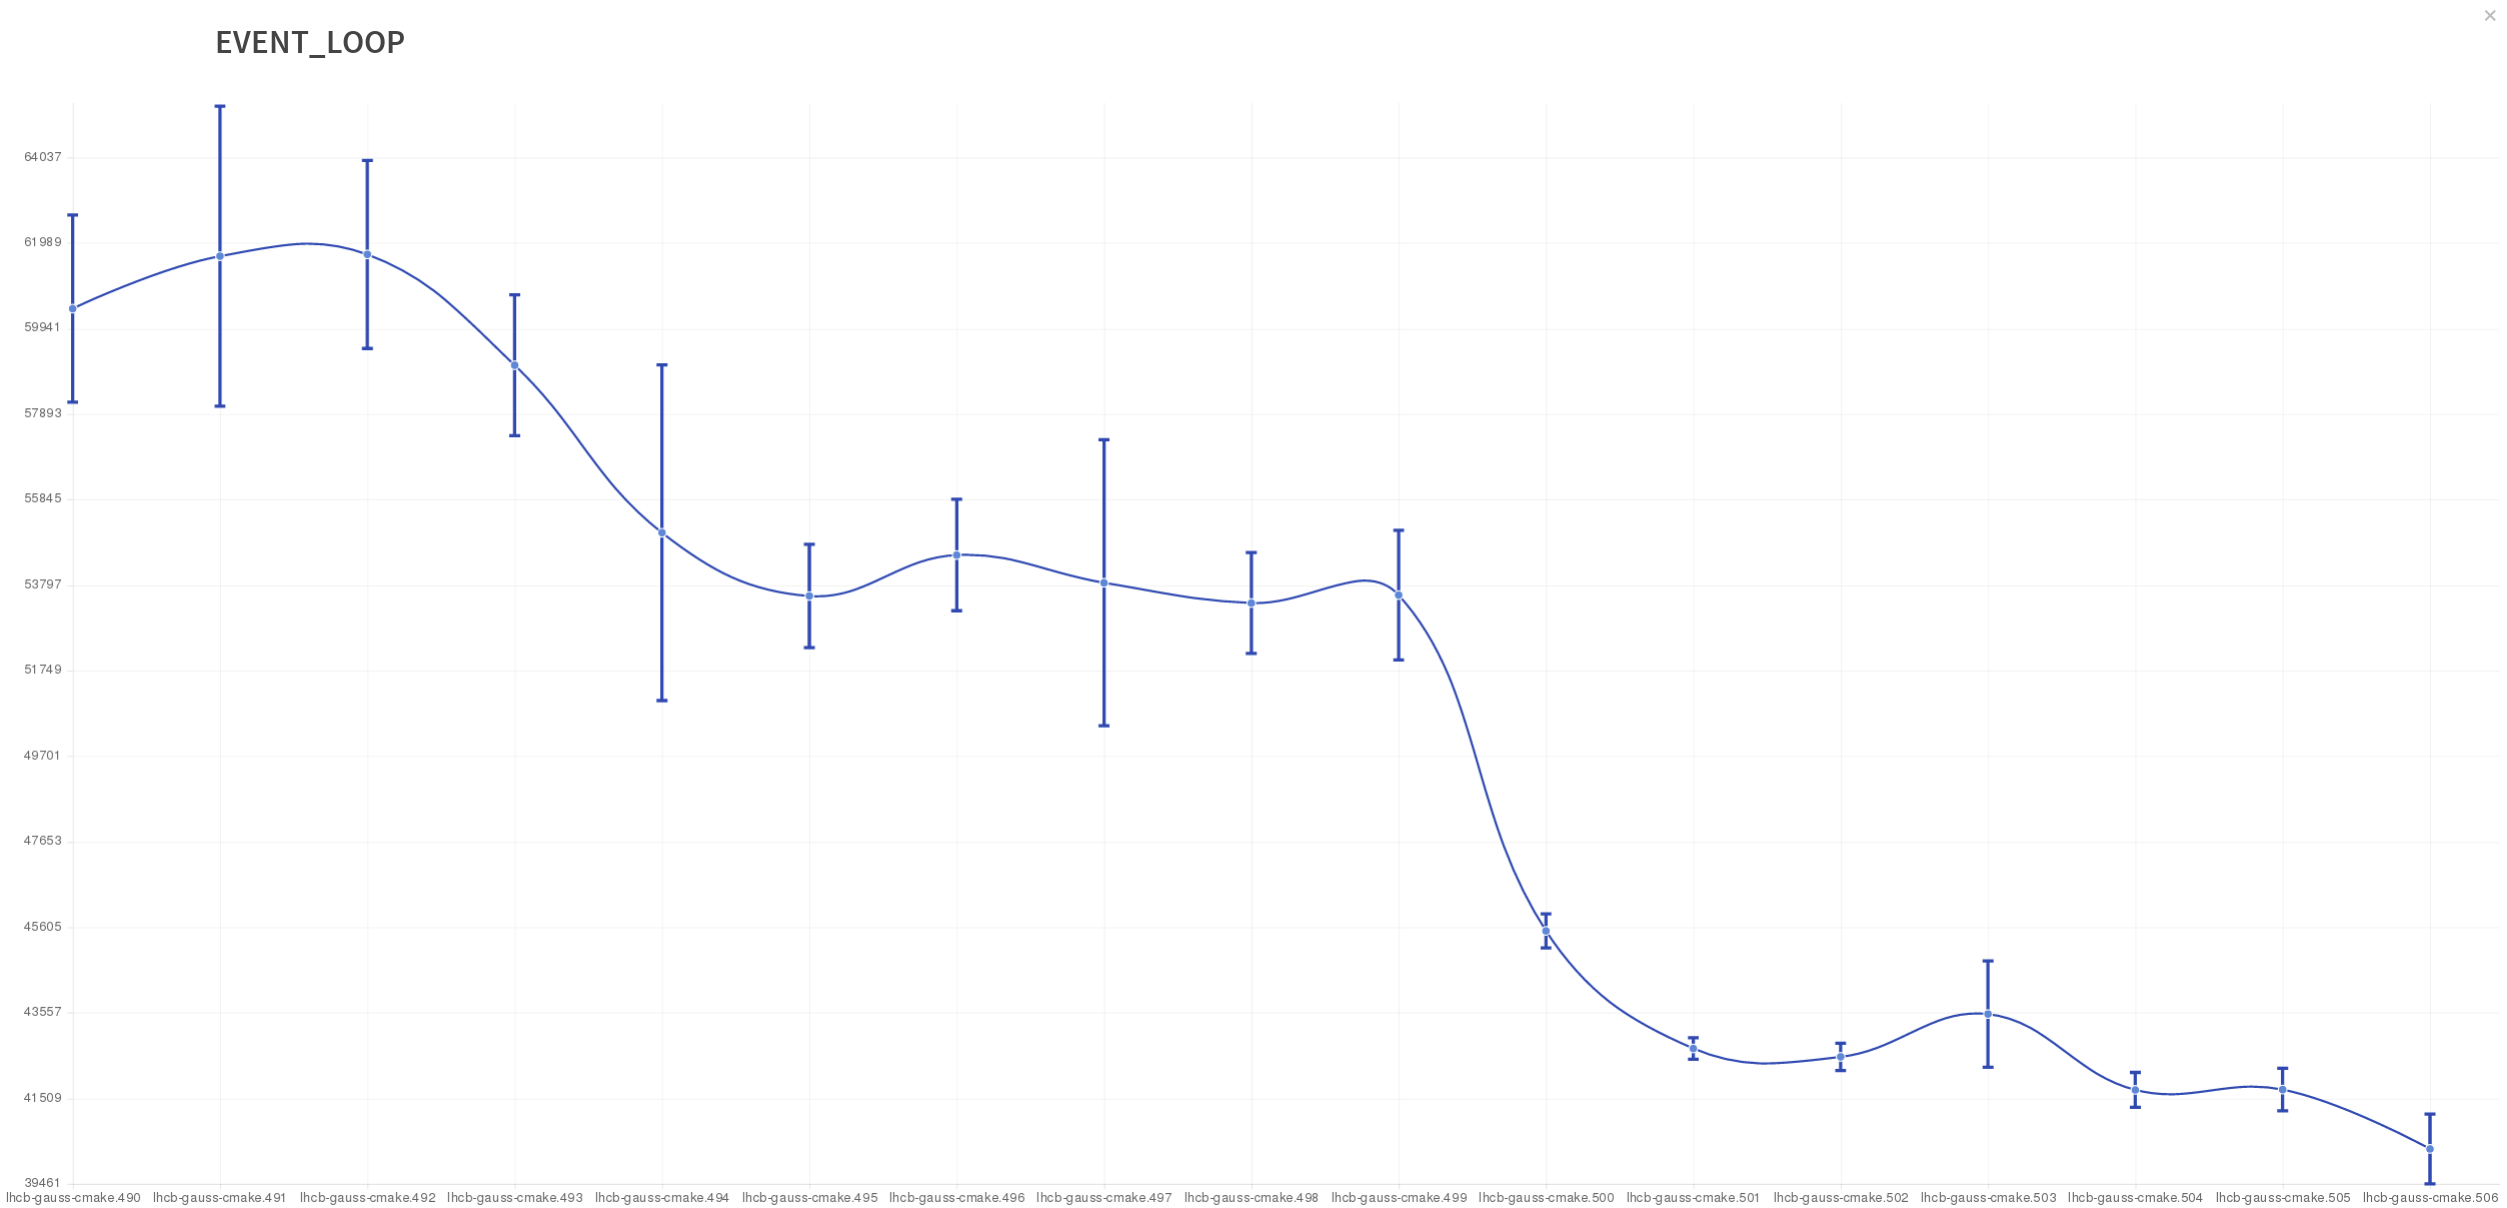
\includegraphics[width=0.84\textwidth]{figures/eventlooplb1.png}
%% }
\visible<1->{
\begin{tikzpicture}%%[show background grid] %% Use grid for positioning, then turn off
		\node [inner sep=0pt,above right]
			{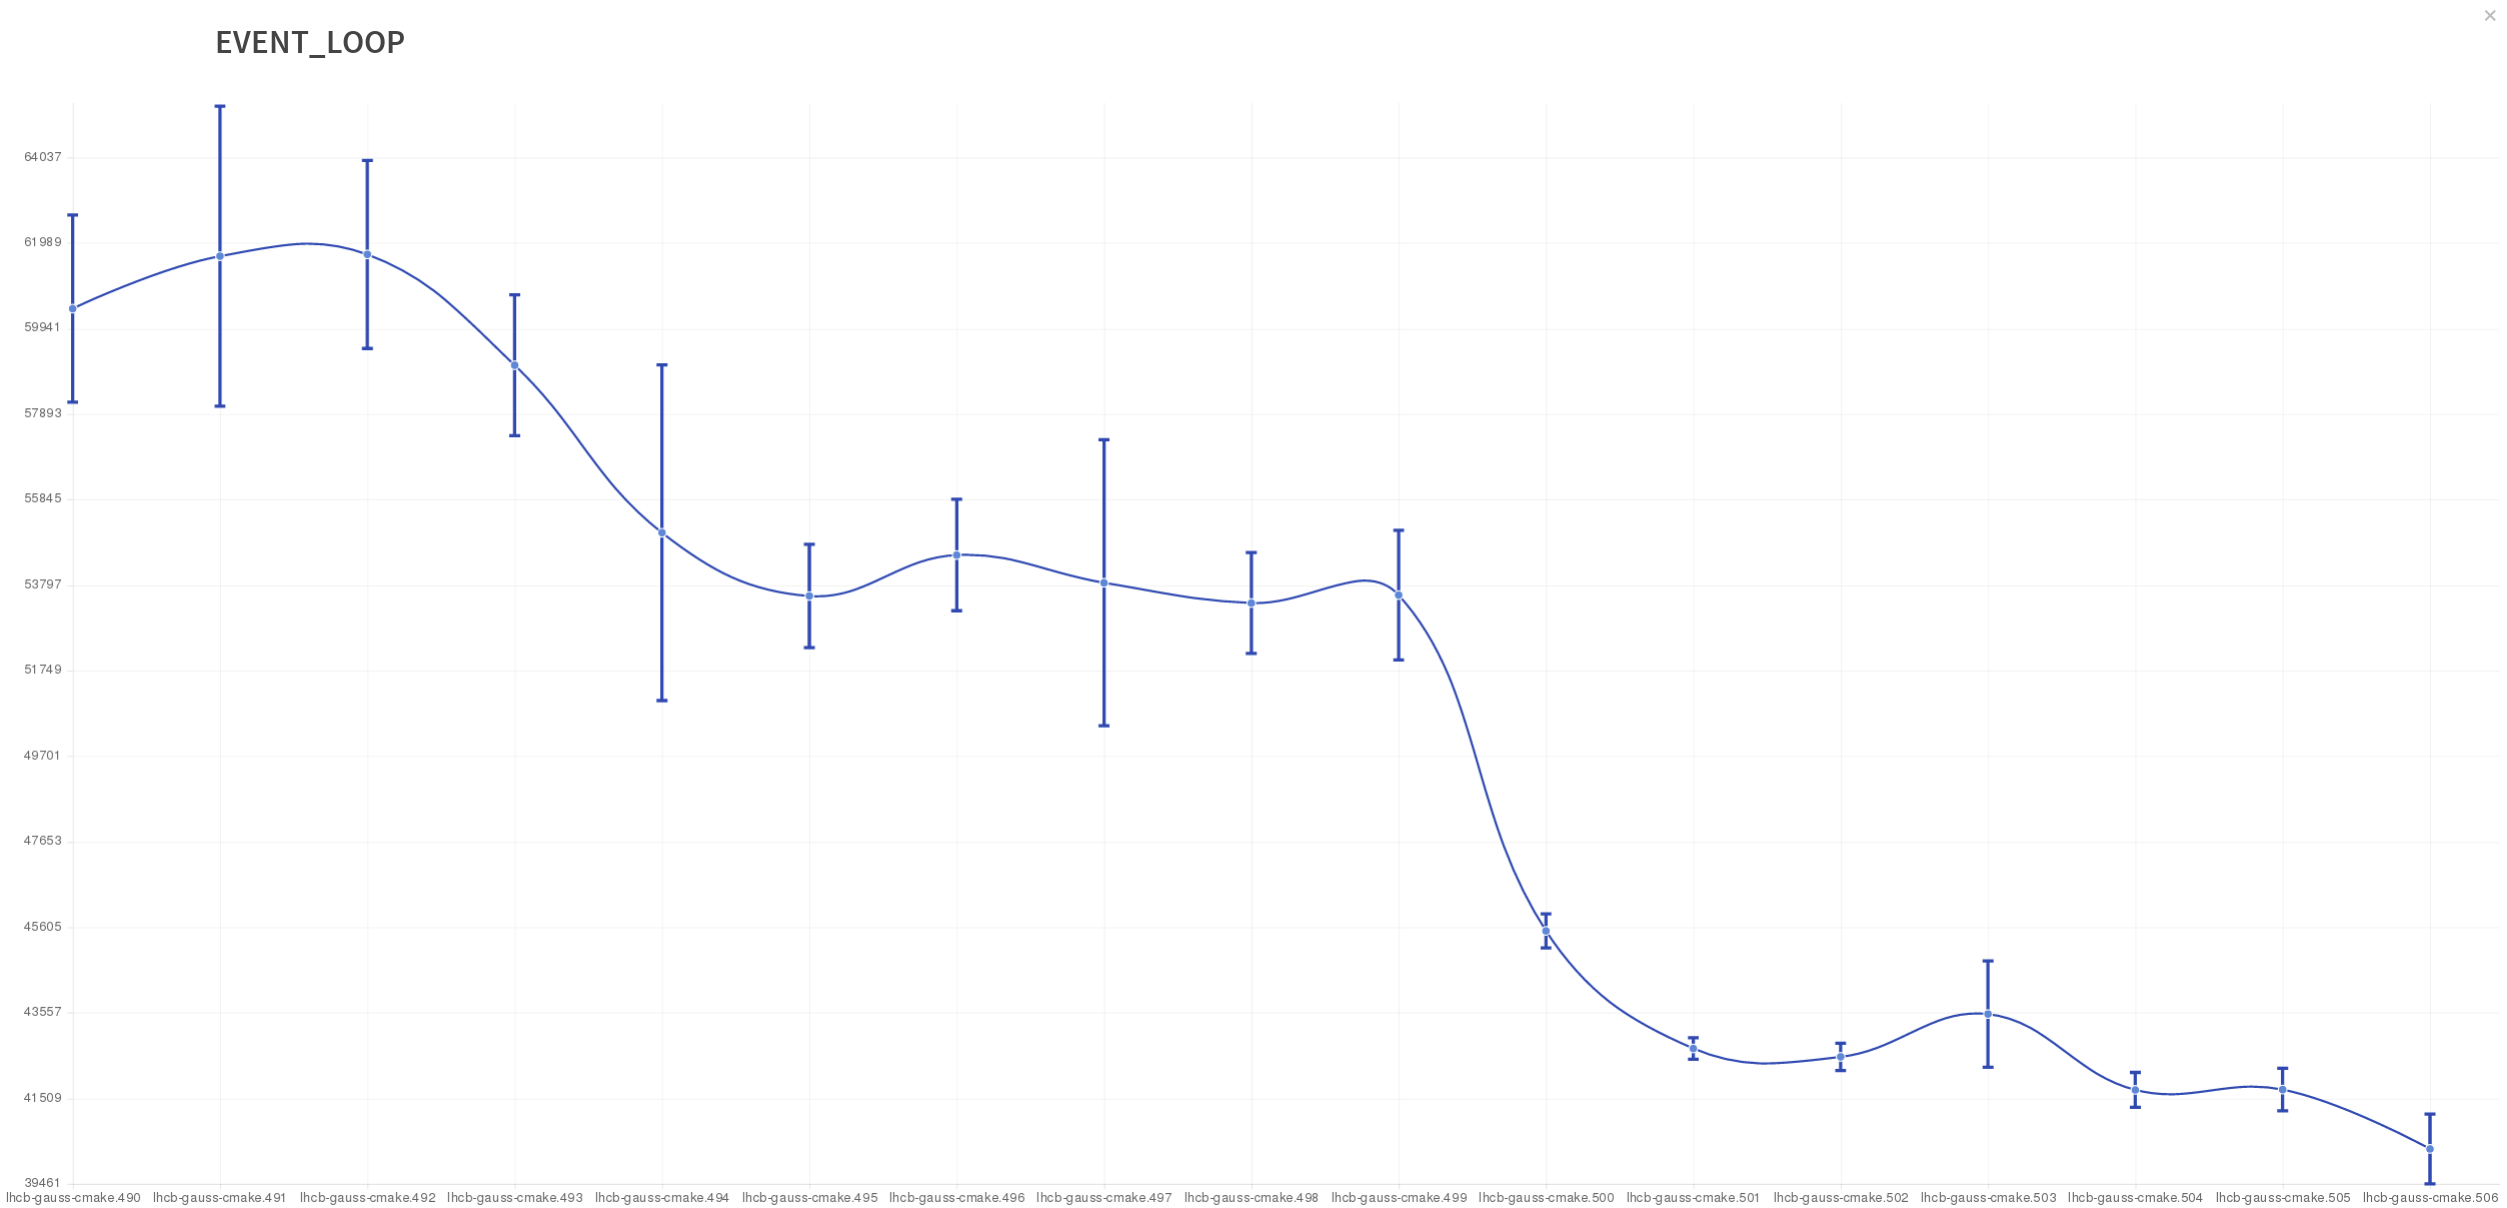
\includegraphics[width=0.8\textwidth]{figures/eventlooplb1.png}};
		\node[right] (blu) at (3.2,4) {\scriptsize\textcolor{blue}{\href{https://gitlab.cern.ch/lhcb/Gauss/merge_requests/164}{\beamergotobutton{Gauss!164}} (RICH fast options)}};
		 \node (bludot) at (2.6,3.3) {};
		 \path[->, color=blue, line width=1] (blu) edge [out = -160, in = 45] (bludot);

		\node[right] (blu) at (8.2,2.5) {\scriptsize\textcolor{blue}{\href{https://indico.cern.ch/event/587955/contributions/2938036/}{\beamergotobutton{Gauss!169}} (new tag)}};
		 \node (bludot) at (6.7,1.7) {};
		 \path[->, color=blue, line width=1] (blu) edge [out = -160, in = 45] (bludot);

		\node[right] (time1) at (0.8,3.2) {\scriptsize\textcolor{blue}{(61.7$\pm$2.3)s}};
		\node[right] (time1) at (2.8,2.0) {\scriptsize\textcolor{blue}{(53.5$\pm$1.2)s}};
		\node[right] (time1) at (10.0,0.8) {\scriptsize\textcolor{blue}{(40.3$\pm$0.8)s}};

\end{tikzpicture}
}

\end{center}
\end{frame}


\begin{frame}[fragile]
\frametitle{\centerline{Using ROOT file viewer}}
\begin{tikzpicture}%[show background grid] %% Use grid for positioning, then turn off
\visible<1>{
		\node [inner sep=0pt,above right] 
			{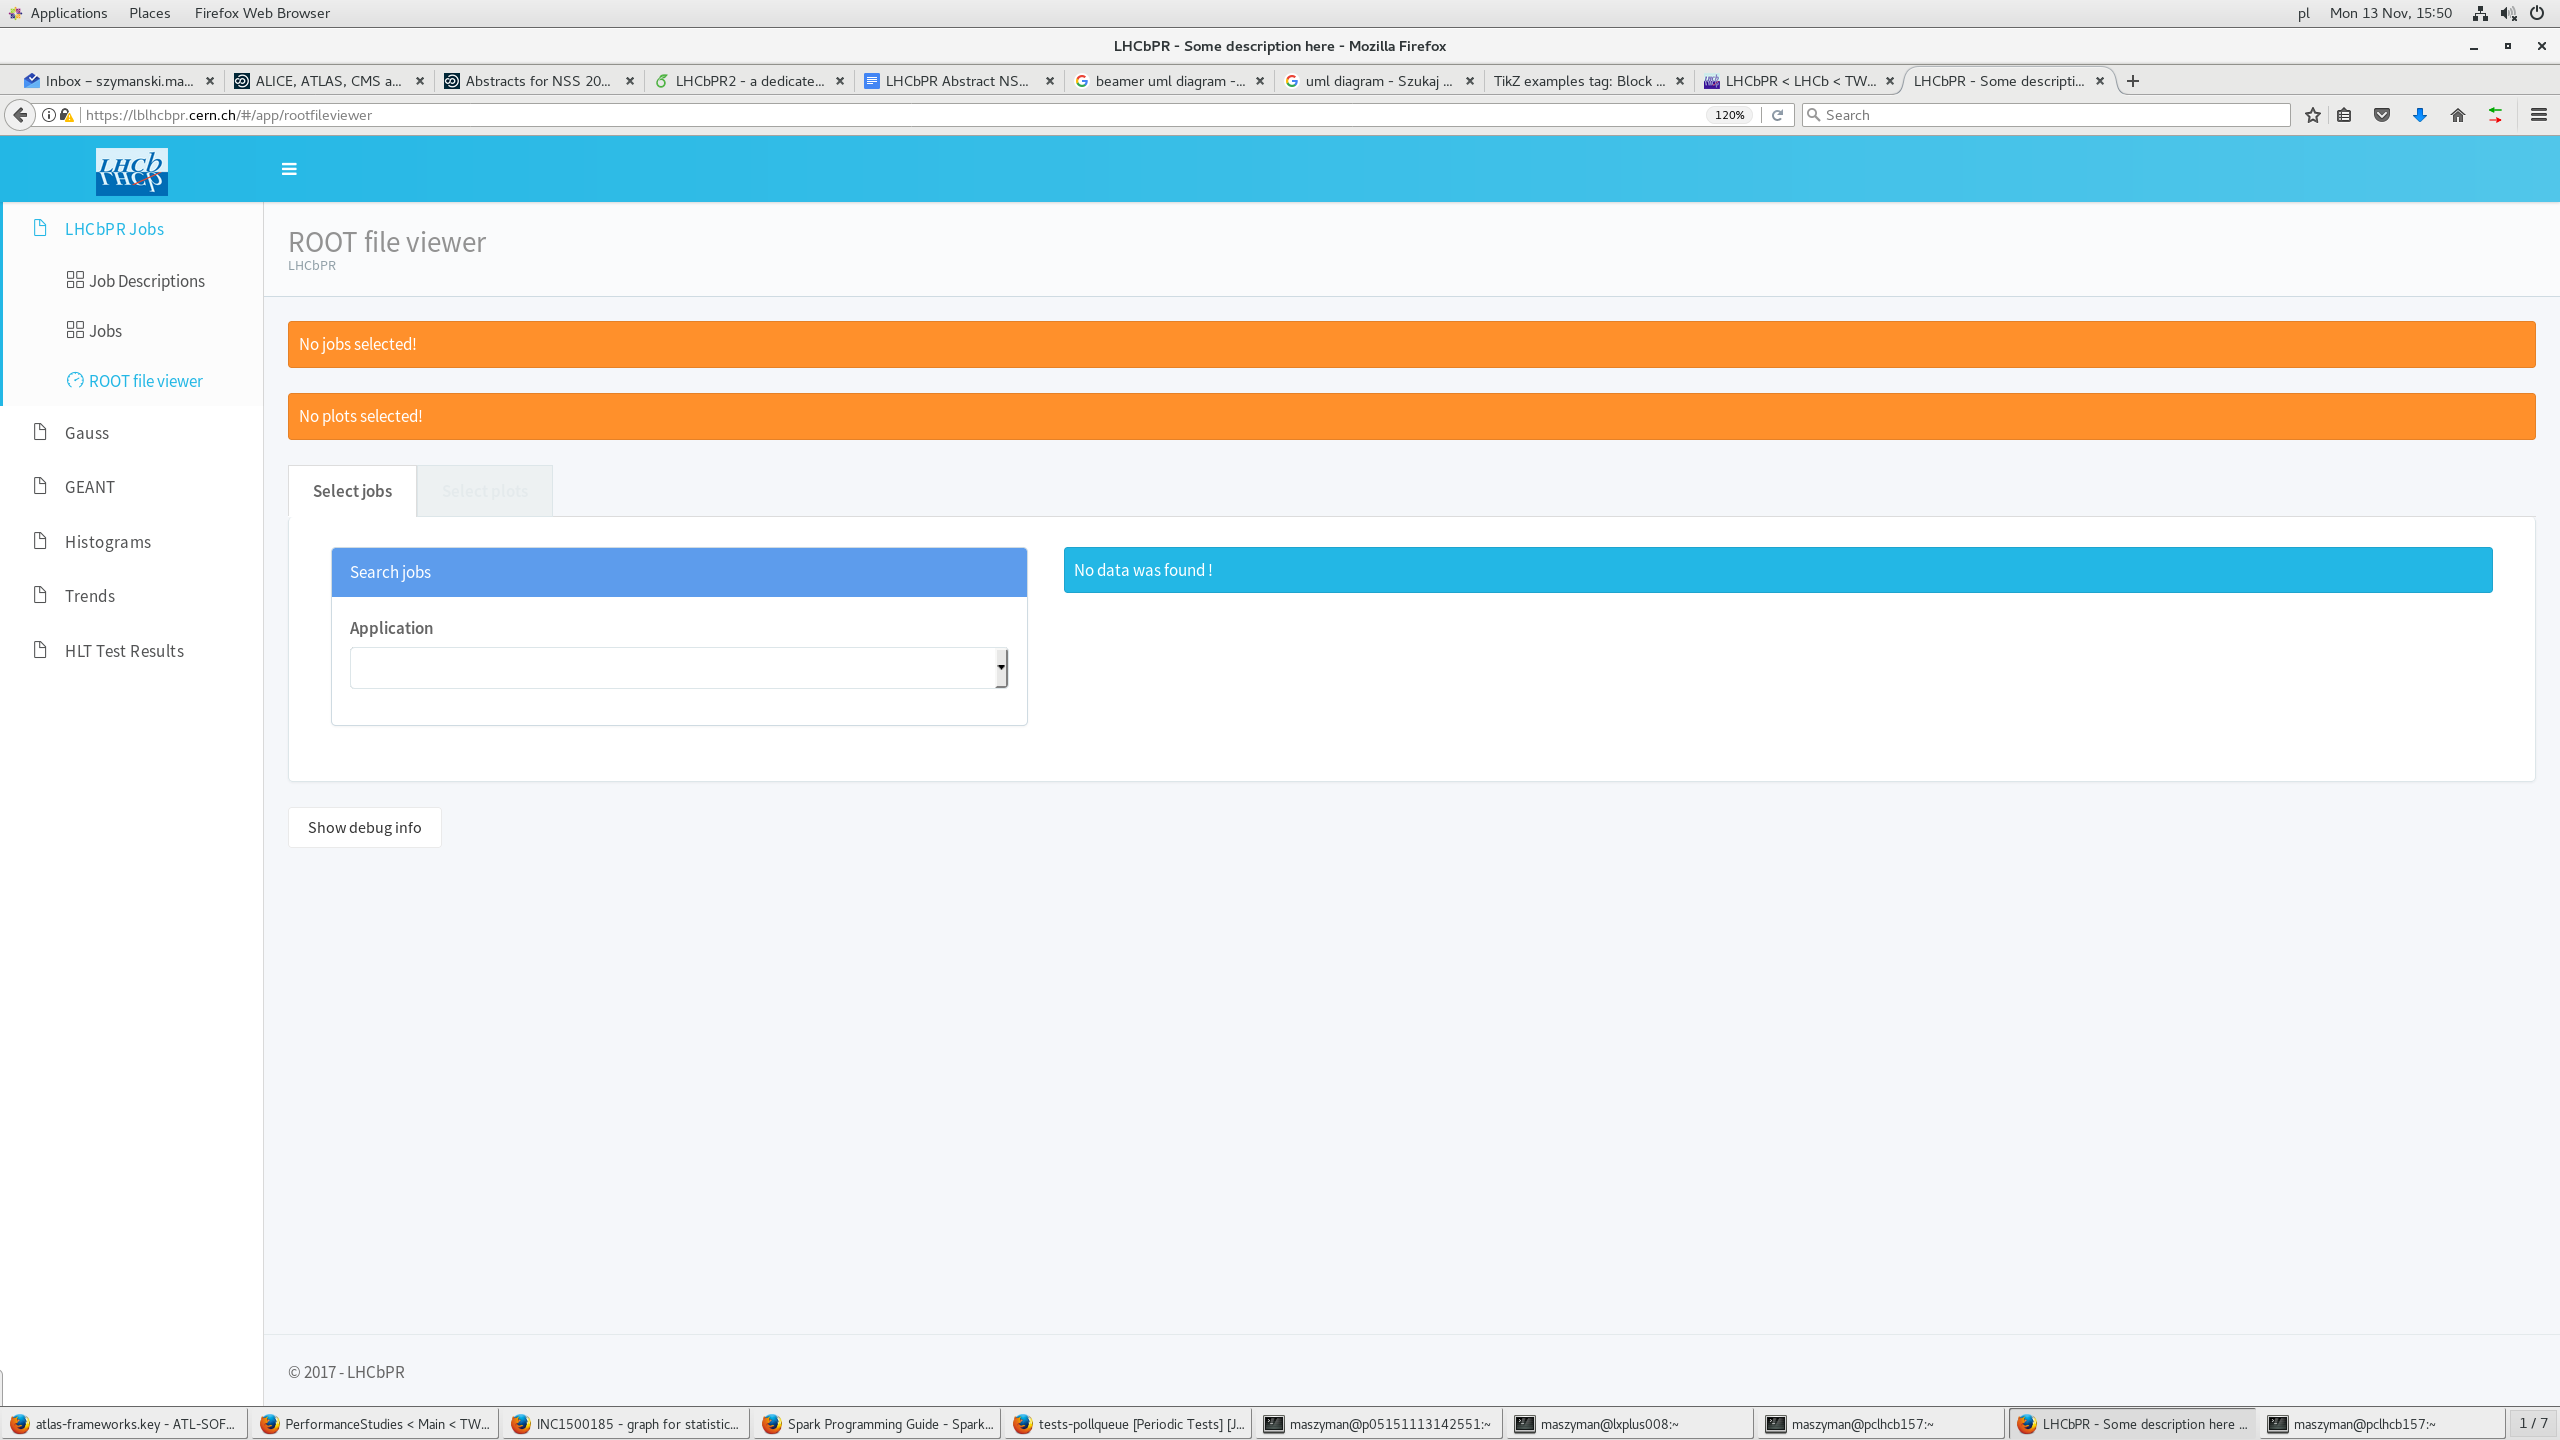
\includegraphics[width=0.99\textwidth]{figures/root1.png}};
}
\visible<2-4>{
		\node [inner sep=0pt,above right] 
			{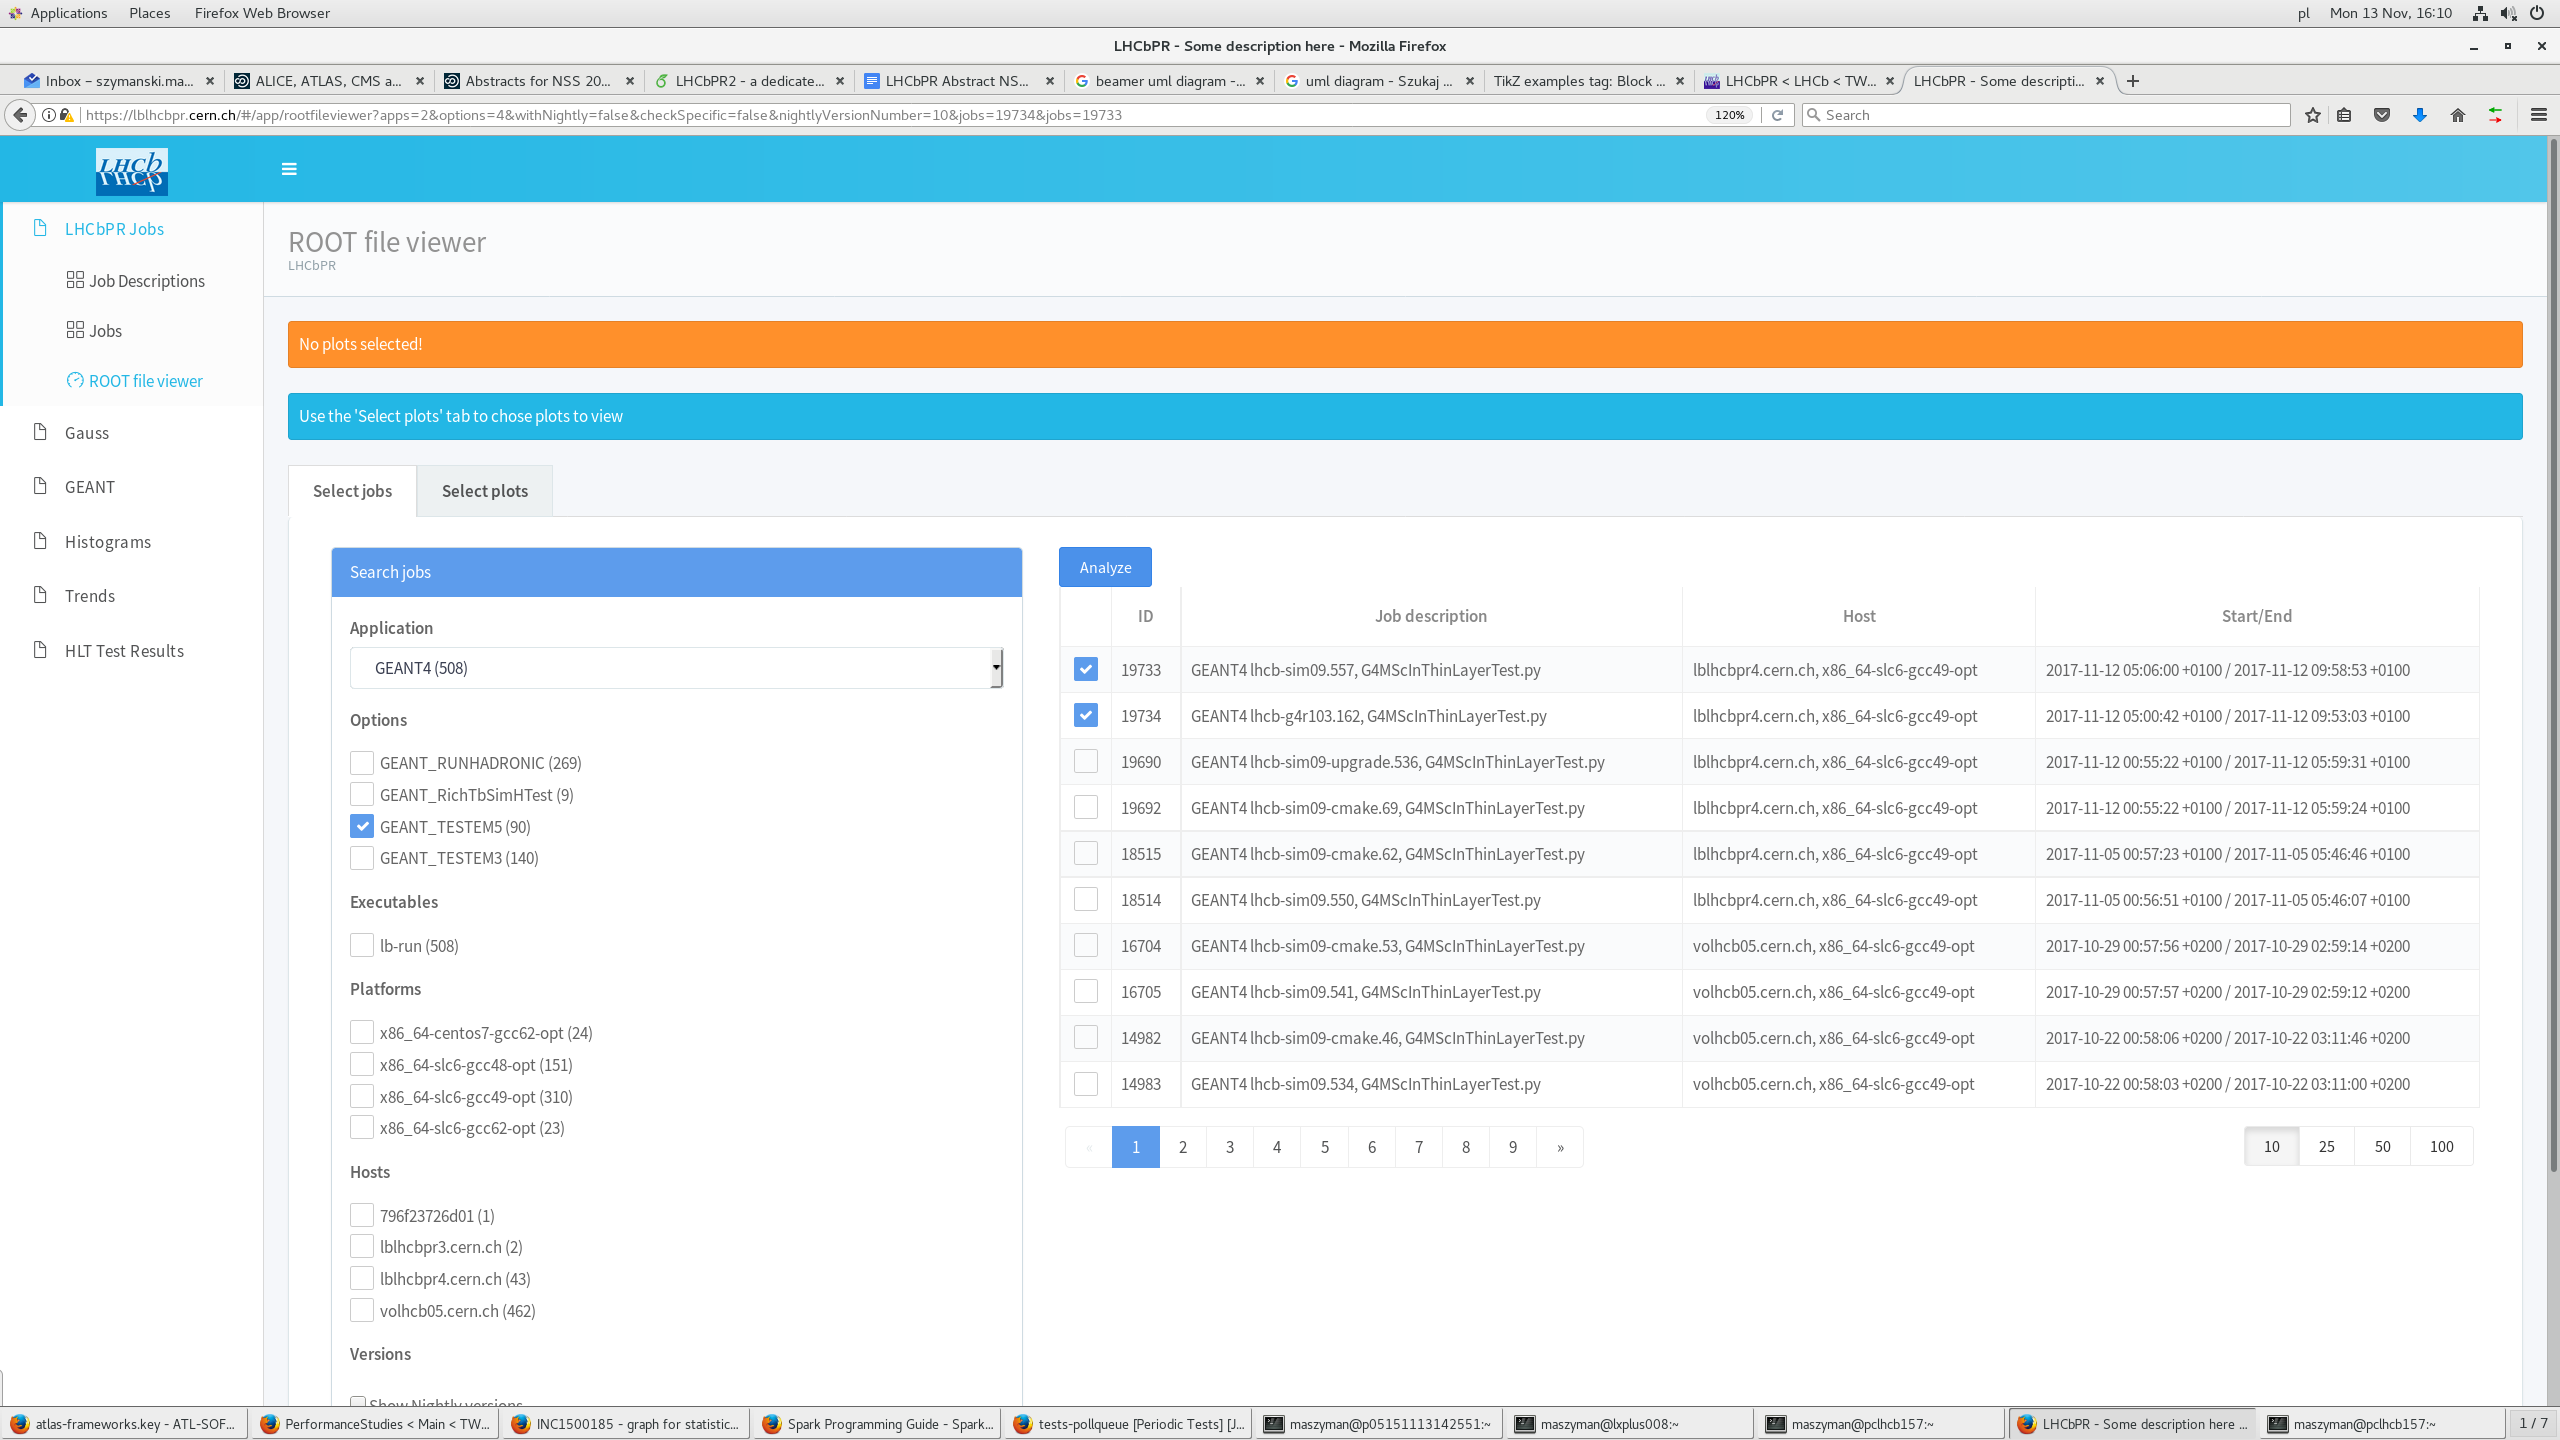
\includegraphics[width=0.99\textwidth]{figures/root2.png}};
}
\visible<5-6>{
		\node [inner sep=0pt,above right] 
			{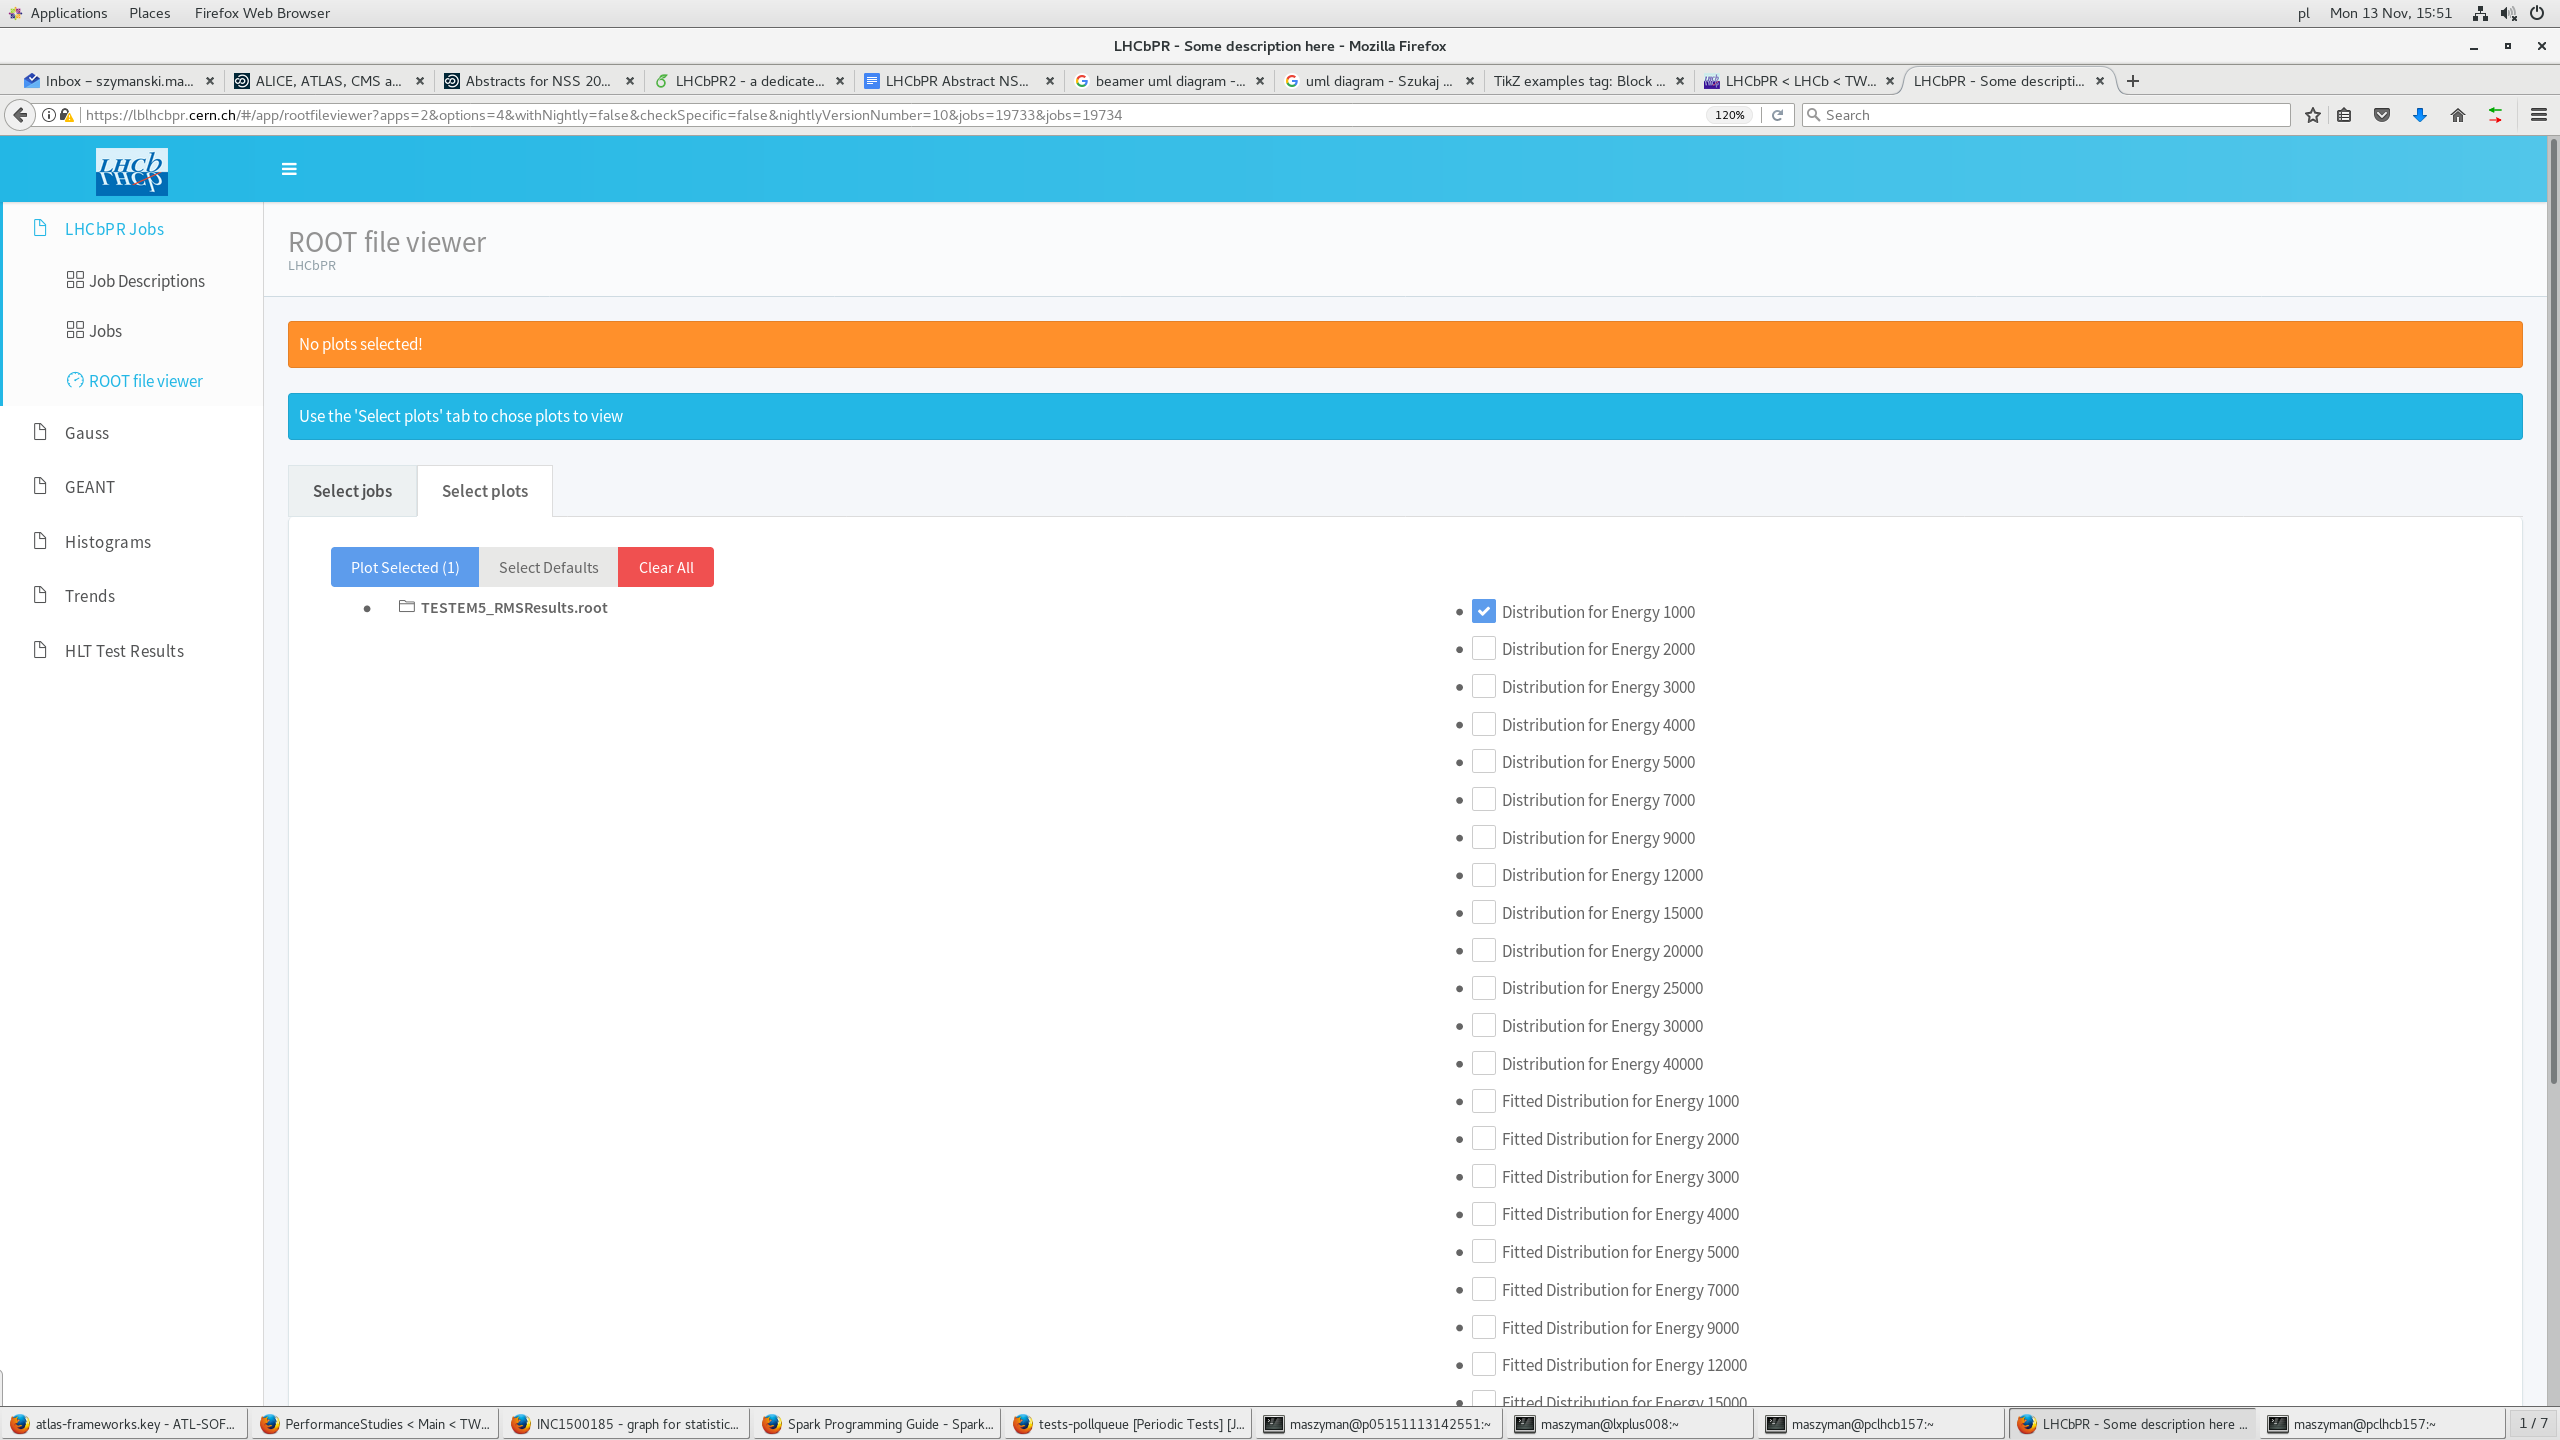
\includegraphics[width=0.99\textwidth]{figures/root4.png}};
}
\visible<6>{
		\node [inner sep=0pt,above right] 
			{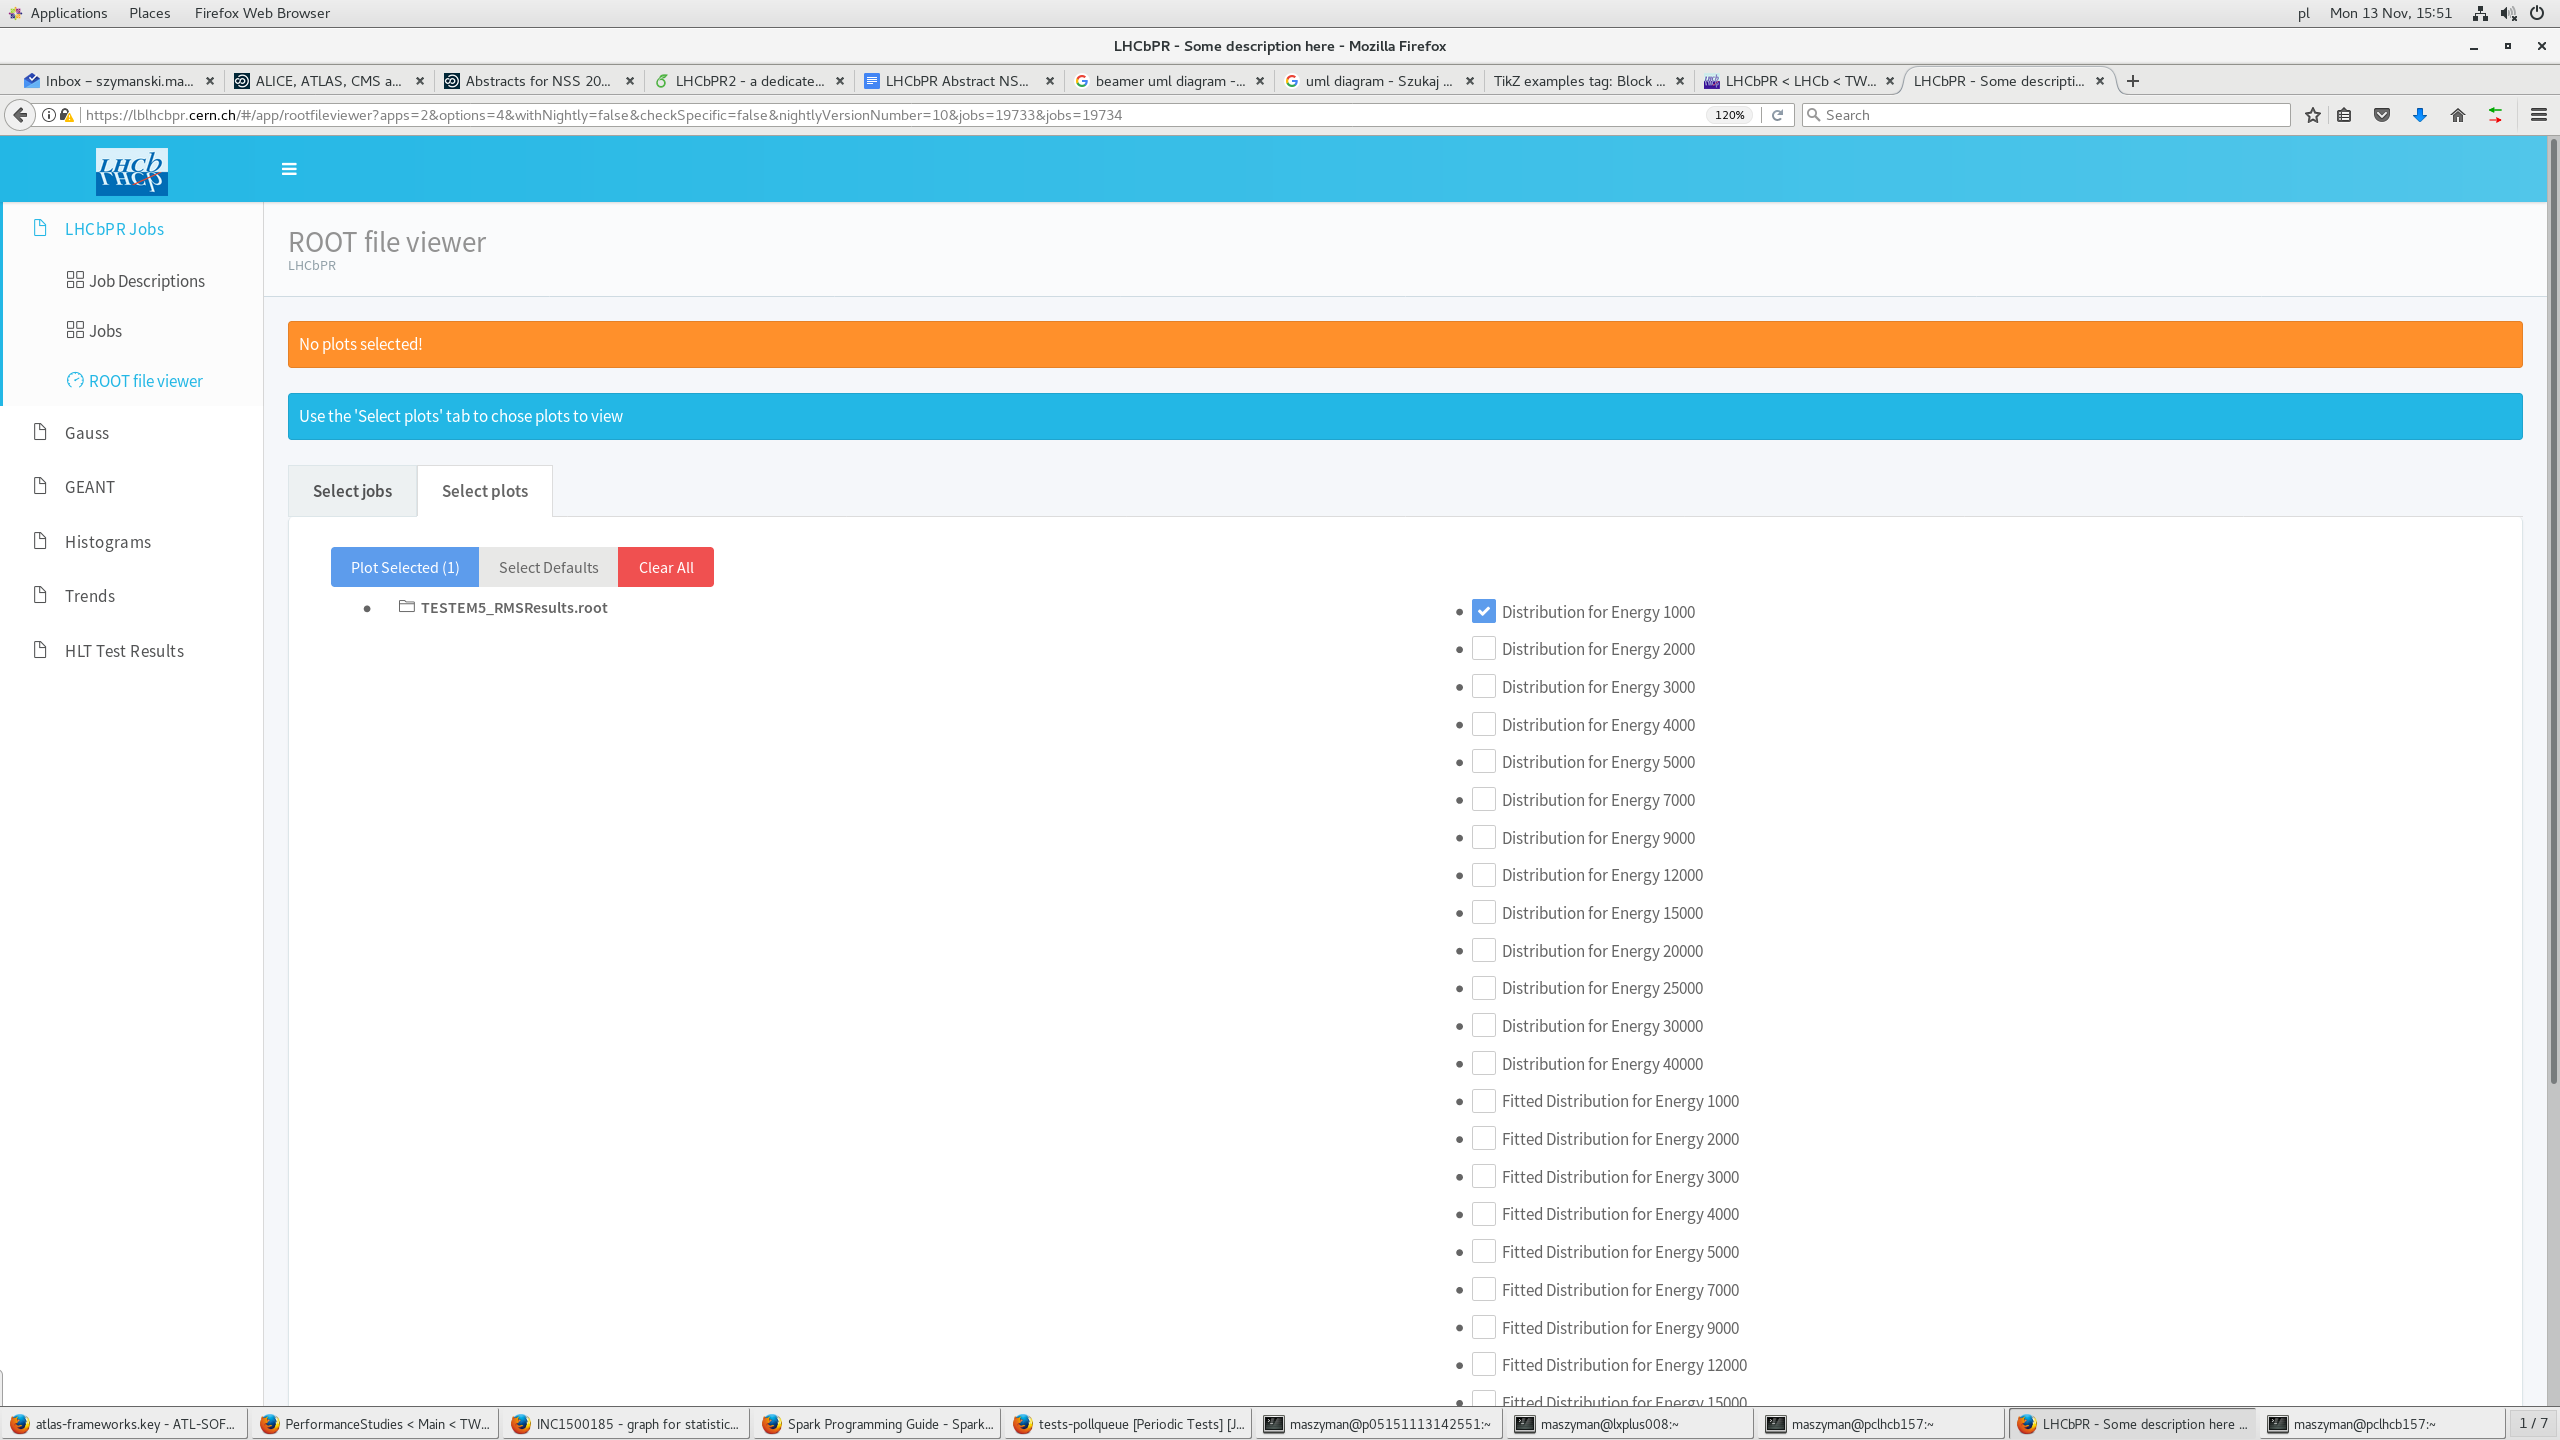
\includegraphics[width=0.99\textwidth]{figures/root4.png}};
}
\visible<7>{
		\node [inner sep=0pt,above right] 
			{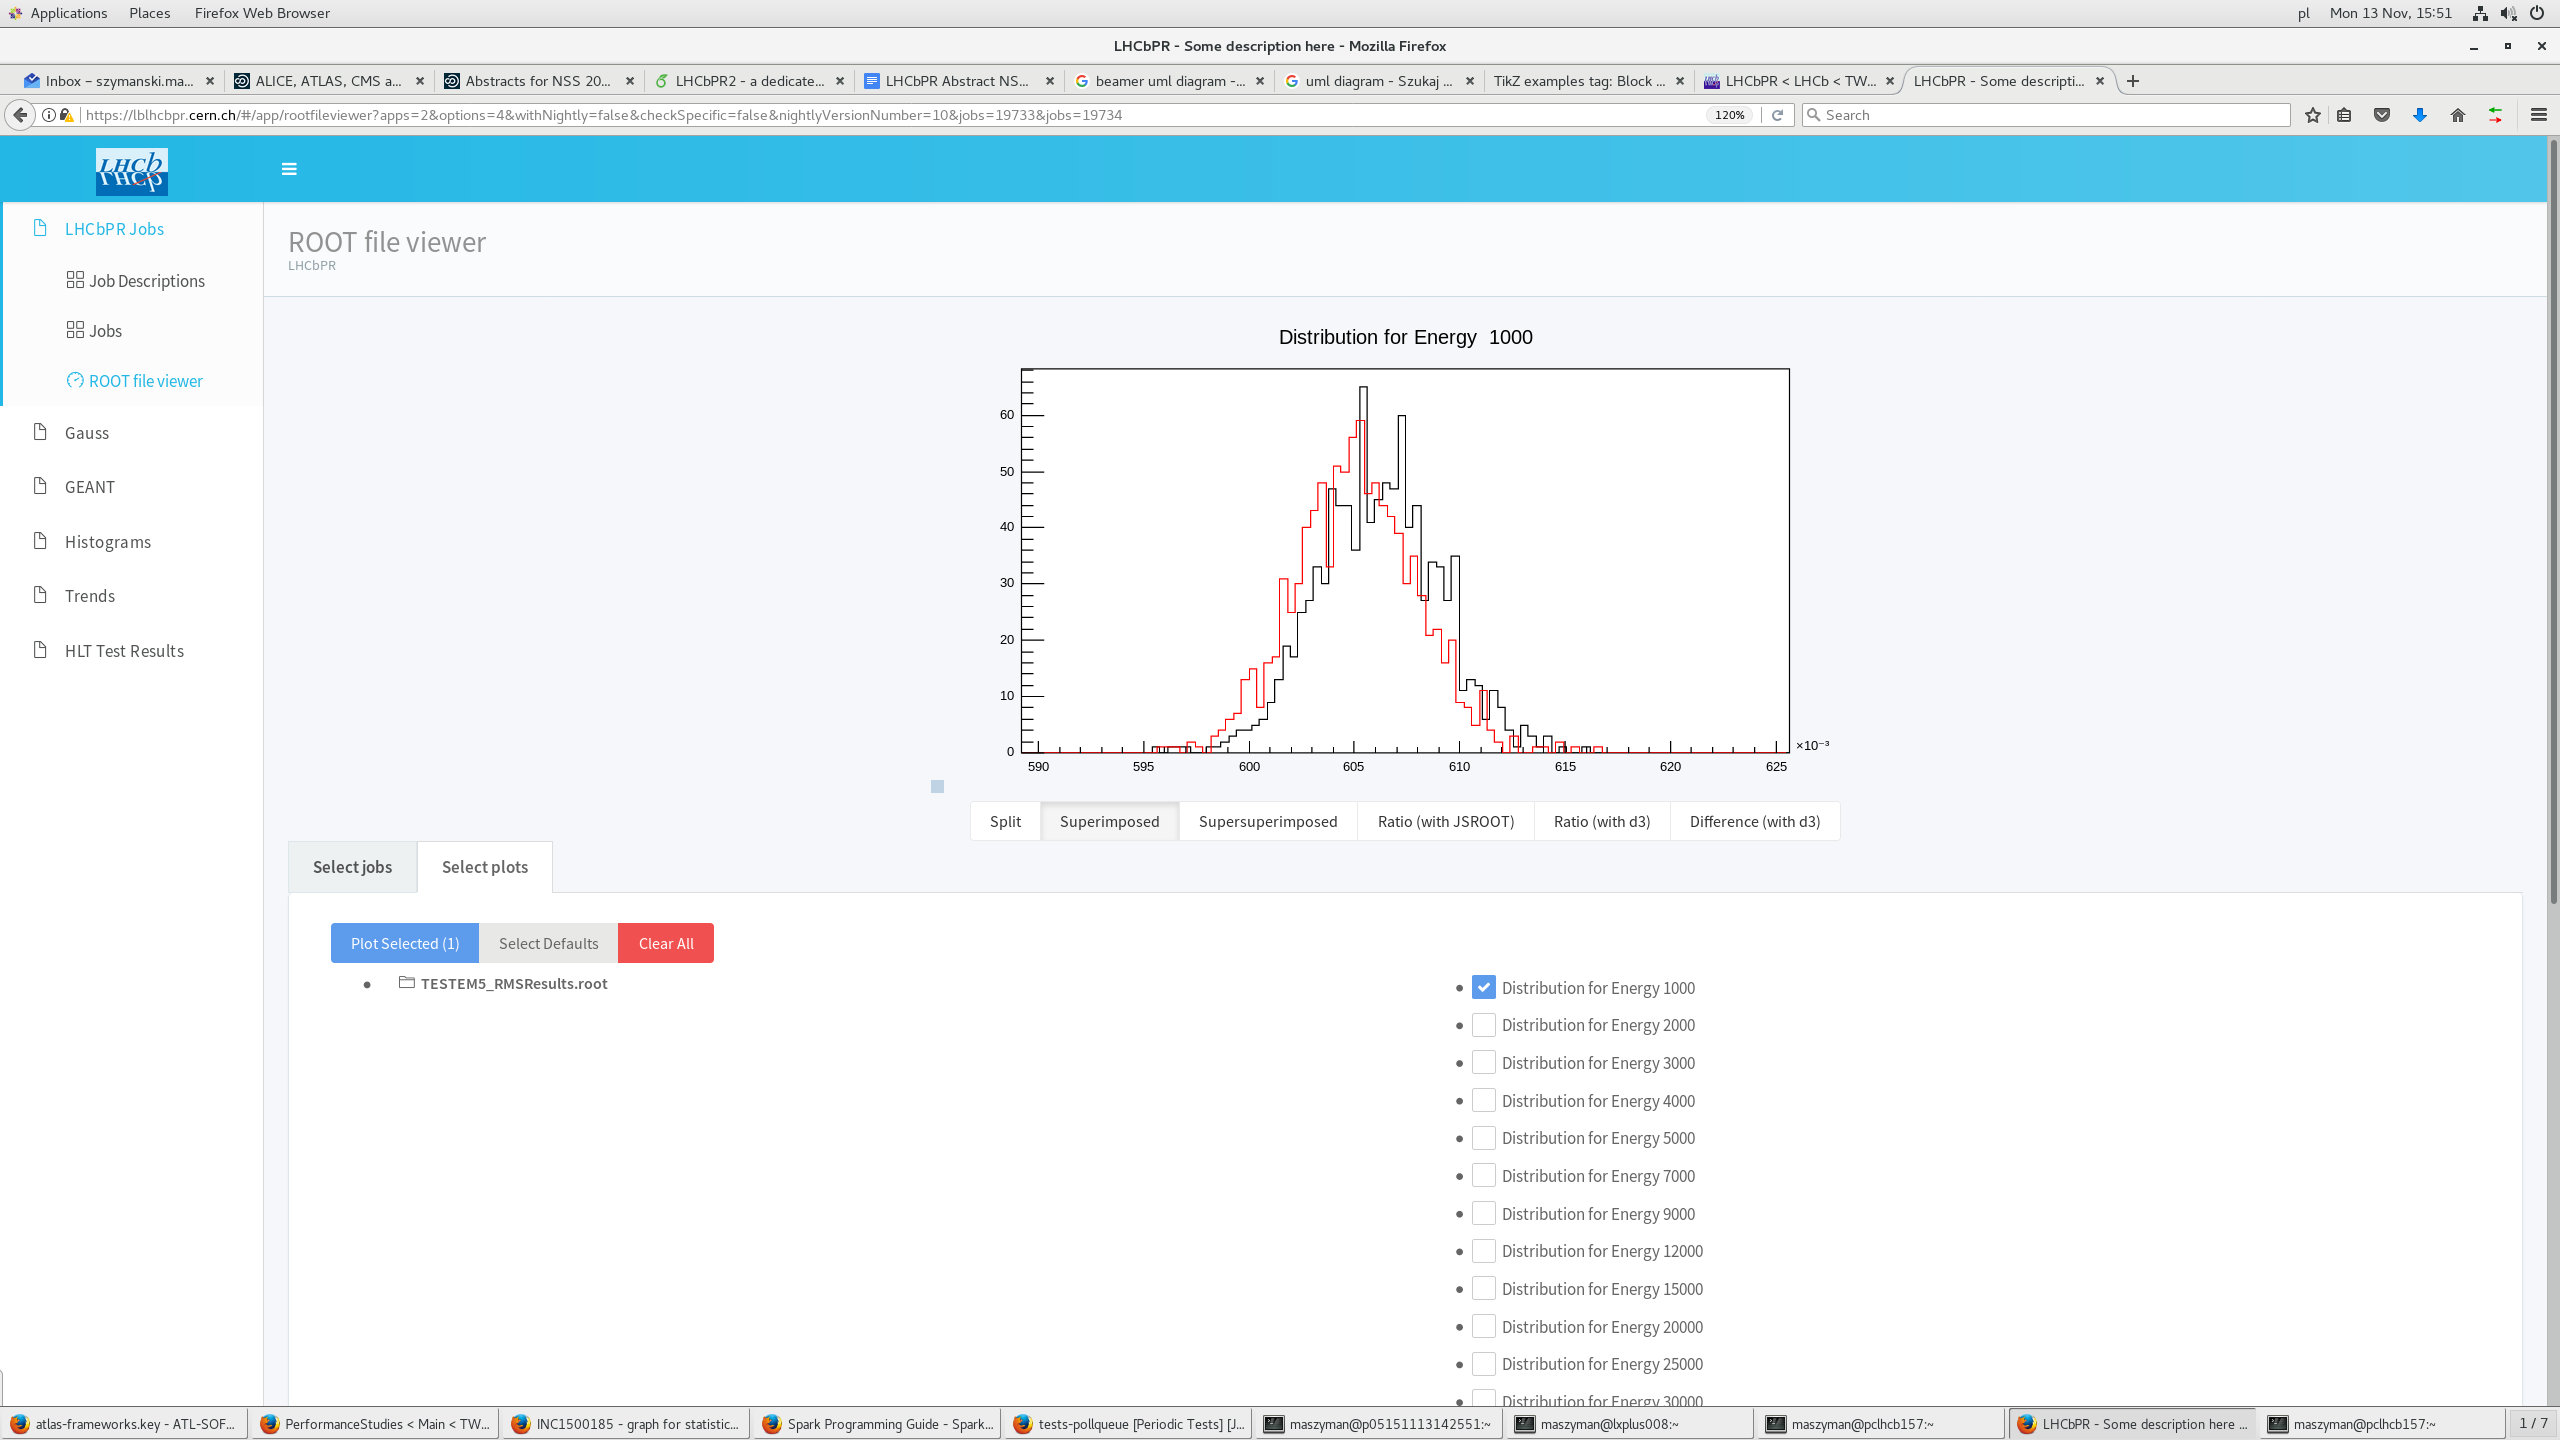
\includegraphics[width=0.99\textwidth]{figures/root5.png}};
}
\visible<1>{
		\node[right] (blu1) at (6,3) {\scriptsize\textcolor{blue}{go to {\it LHCbPR Jobs/ROOT file viewer} tab}};
}
\visible<2>{
		\node[right] (blu2) at (6,5) {\scriptsize\textcolor{blue}{select applications, filter options etc}};
}
\visible<3>{
		\node[right] (blu3) at (8,5) {\scriptsize\textcolor{blue}{select jobs to analyze and click {\it Analyze}}};
}
\visible<4>{
		\node[right] (blu4) at (8,5) {\scriptsize\textcolor{blue}{click on {\it Select plots}}};
}
\visible<5>{
		\node[right] (blu5) at (5,3) {\scriptsize\textcolor{blue}{select your histogram}};
}
\visible<6>{
		\node[right] (blu6) at (5,3) {\scriptsize\textcolor{blue}{click on {\it Plot selected} }};
}
\visible<7>{
		\node[right] (blu7) at (10,4.5) {\scriptsize\textcolor{blue}{choose the way of display}};
}
		 \node (bludot1) at (0.8,5.7) {};
		 \node (bludot2) at (2.8,4.1) {};
		 \node (bludot3) at (5.9,4.3) {};
		 \node (bludot4) at (2.8,5.1) {};
		 \node (bludot5) at (8.2,4.6) {};
		 \node (bludot6) at (2.2,4.6) {};
		 \node (bludot7) at (6.2,3.2) {};
\visible<1>{
		 \path[->, color=blue, line width=1] (blu1) edge [out = 160, in = 45] (bludot1);
}
\visible<2>{
		 \path[->, color=blue, line width=1] (blu2) edge [out = 160, in = 45] (bludot2);
}
\visible<3>{
		 \path[->, color=blue, line width=1] (blu3) edge [out = 160, in = 45] (bludot3);
}
\visible<4>{
		 \path[->, color=blue, line width=1] (blu4) edge [out = 160, in = 45] (bludot4);
}
\visible<5>{
		 \path[->, color=blue, line width=1] (blu5) edge [out = 160, in = 45] (bludot5);
}
\visible<6>{
		 \path[->, color=blue, line width=1] (blu6) edge [out = 160, in = 45] (bludot6);
}
\visible<7>{
		 \path[->, color=blue, line width=1] (blu7) edge [out = 160, in = 45] (bludot7);
}
\end{tikzpicture}

\end{frame}



\begin{frame}% [<+->]
%% {About me}
\frametitle{\centerline{Upgrade benchmarking}}
\begin{itemize}
\footnotesize
\setlength\itemsep{10pt}
\item<1-> Special case for the upgrade studies
\item<1-> Tests results pushed to eos website: \url{ https://cern.ch/lhcbpr-hlt/PerfTests/UpgradeVelo}
\item<1-> Throughput test (Velo only and best performance)
\item<1-> PrChecker (Velo only)
\item<1-> Running on \texttt{lhcb-tdr-test} (\texttt{HEAD} of everything)
\item<1-> Notifications when results available sent to mattermost private channel (please let us know if you're interested)
\item<1-> More tests to come
\end{itemize}
\end{frame}

 \begin{frame}% [<+->]
% %% {About me}
 \frametitle{\centerline{Perf test for Gauss	}}
\begin{itemize}
\footnotesize
 \item  Linux tool integrated in the kernel to (see \href{https://twiki.cern.ch/twiki/bin/view/LHCb/CodeAnalysisTools\#Linux_perf_also_known_as_perf_ev}{\beamergotobutton{tutorial by Hadrien}}):
\begin{itemize}
\scriptsize
\item measure CPU statistics
\item investigate where the program spends time
\item produce call graphs
\end{itemize}

\item Test runs with command:

\texttt{
perf record --call-graph=lbr -o perf.log lb-run -c \{platform\} --user-area=\{build\} \{app\_name\}/\{app\_version\} gaudirun.py \{options\}
}

\texttt{
perf report -i perf.log > perf.lbr.txt
}
\item Using lhcb-sim09-upgrade and \$PRCONFIGOPTS/Gauss/PRTEST-2016-SIM-P8-10000000-100evts.py
\item Scheduled to run weekly in LHCbPR
\item Example of results:

\tiny \url{https://lblhcbpr.cern.ch/\#/app/jobs/list?apps=4\&executables=13\&withNightly=false\&checkSpecific=false\&nightlyVersionNumber=10\&jobs=47746\&ssf=false}
 \end{itemize}

\end{frame}

\begin{frame}
\centering
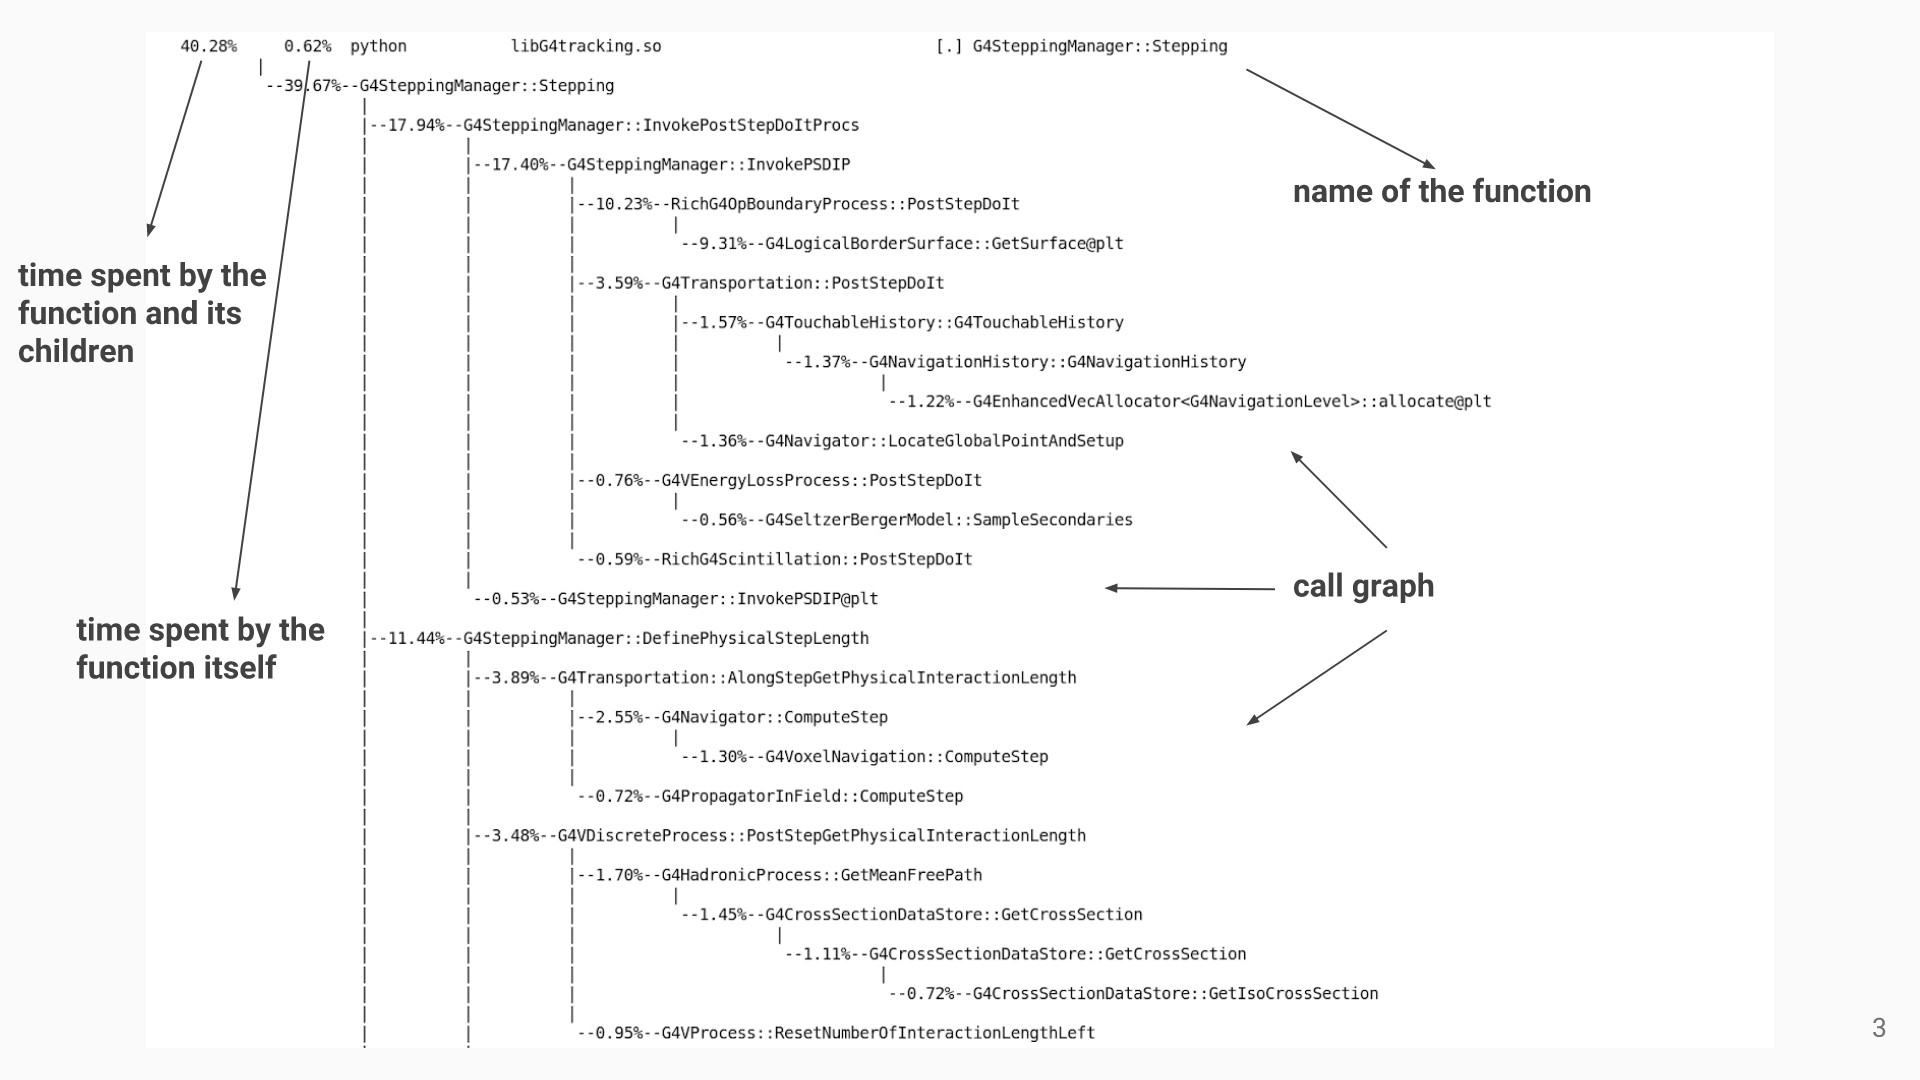
\includegraphics[width=1.09\textwidth]{perf.png}
\end{frame}

\begin{frame}
\frametitle{\centerline{Flame graph}}
%\centering
\vskip 2pt
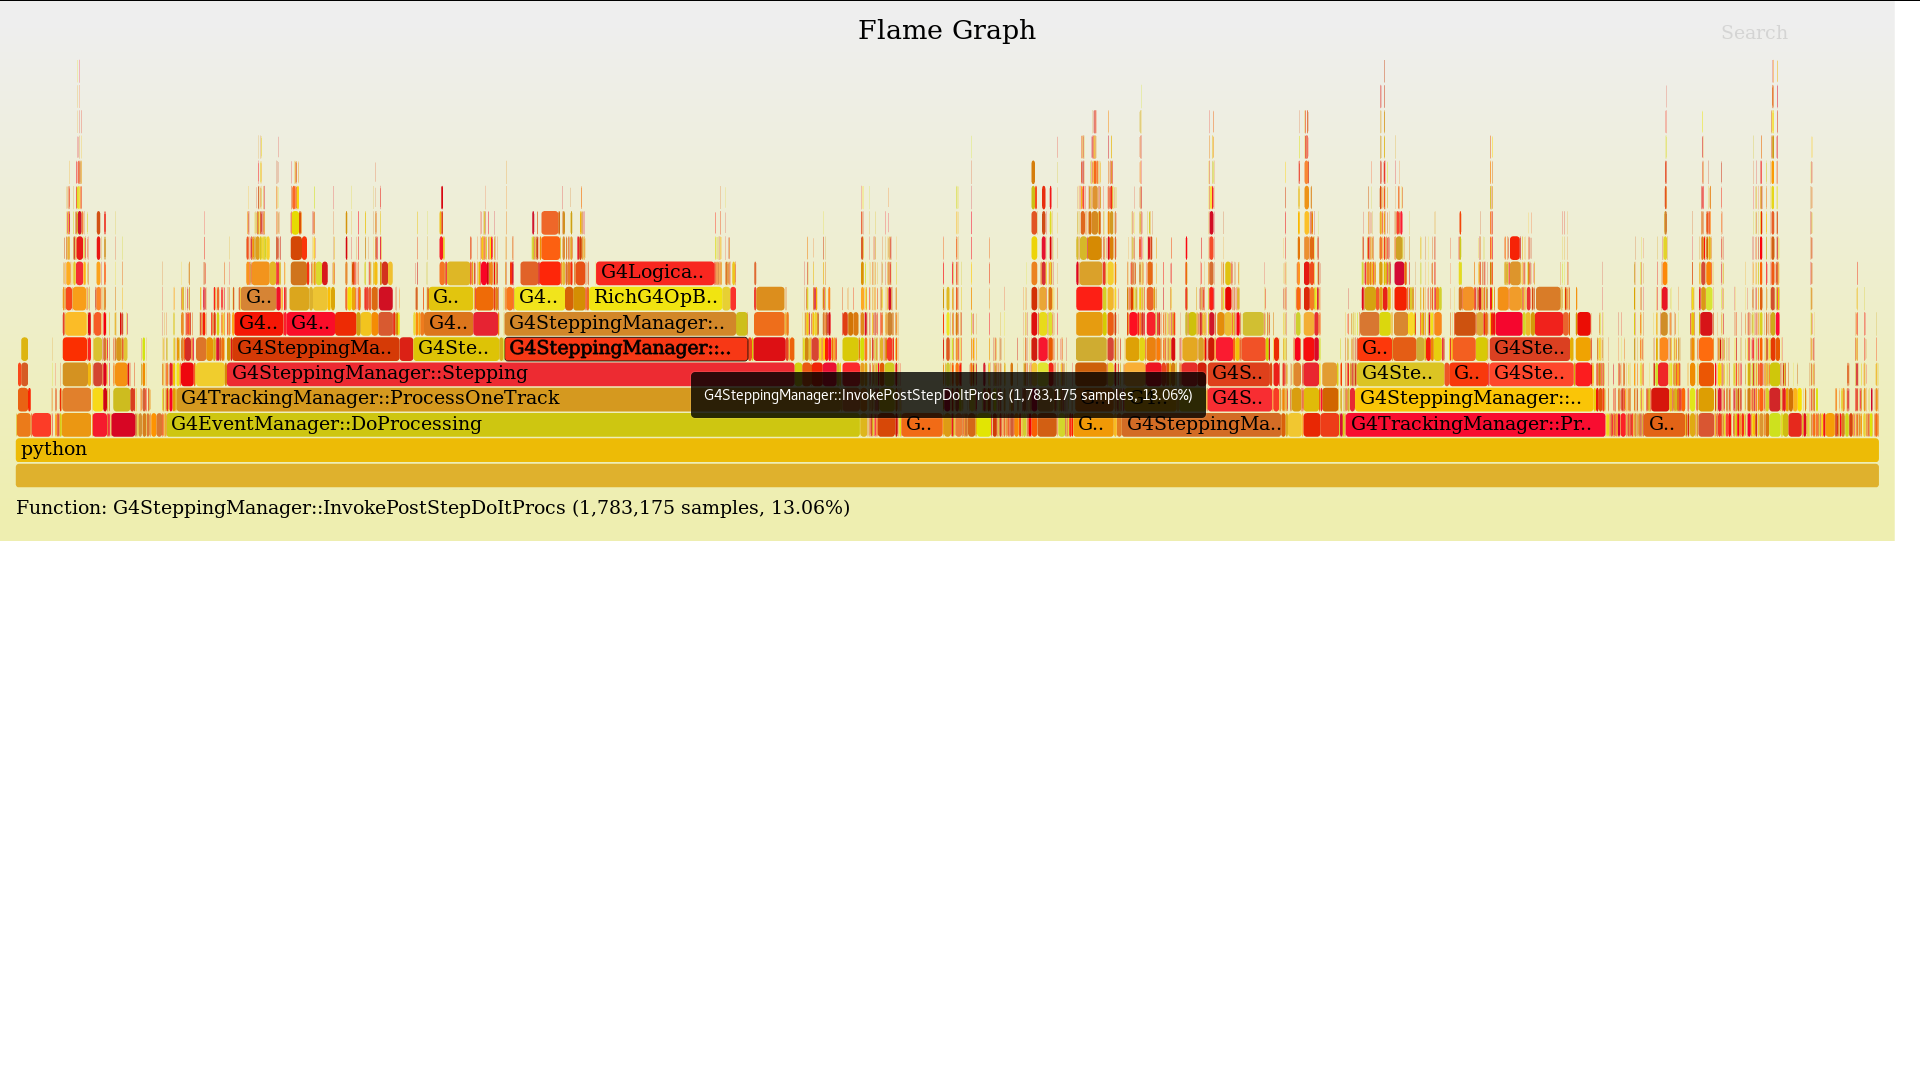
\includegraphics[width=1.49\textwidth]{flame.png}
\end{frame}

\begin{frame}% [<+->]
%% {About me}
\frametitle{\centerline{Igprof test for Gauss	}}
\begin{itemize}
\footnotesize
\item Performance and memory profiling tool, here just focus on:
\begin{itemize}
\scriptsize
\item memory that hasn’t be freed
\item total memory allocated by any function
\end{itemize}
\item Test runs with command:

\texttt{
igprof\_env="lb-run -c \{platform\} --ext igprof --user-area=\{build\} \{app\_name\}/\{app\_version\}"
}

\texttt{
\$igprof\_env igprof -d -mp -z -o igout.mp.gz gaudirun.py \{options\}
}

\texttt{
\$igprof\_env igprof-analyse -v -g -r MEM\_LIVE igout.mp.gz > igout.mp.live.txt
}

\texttt{
\$igprof\_env igprof-analyse -v -g -r MEM\_TOTAL igout.mp.gz > igout.mp.total.txt
}
% % igprof\_env="lb-run -c \{platform\} --ext igprof --user-area=\{build\} \{app\_name\}/\{app\_version\}"

% % \$igprof\_env igprof -d -mp -z -o igout.mp.gz gaudirun.py \{options\}

% % \$igprof\_env igprof-analyse -v -g -r MEM\_LIVE igout.mp.gz > igout.mp.live.txt 

% % \$igprof\_env igprof-analyse -v -g -r MEM\_TOTAL igout.mp.gz > igout.mp.total.txt
% ads

\item Using lhcb-sim09-upgrade and \$PRCONFIGOPTS/Gauss/PRTEST-2016-SIM-P8-10000000-100evts.py
\item Scheduled to run weekly in LHCbPR
\item Example of the results:

\tiny \url{https://lblhcbpr.cern.ch/\#/app/jobs/list?apps=4\&executables=14\&withNightly=false\&checkSpecific=false\&nightlyVersionNumber=10\&jobs=30204\&ssf=false}

\end{itemize}
\end{frame}

\begin{frame}
\centering
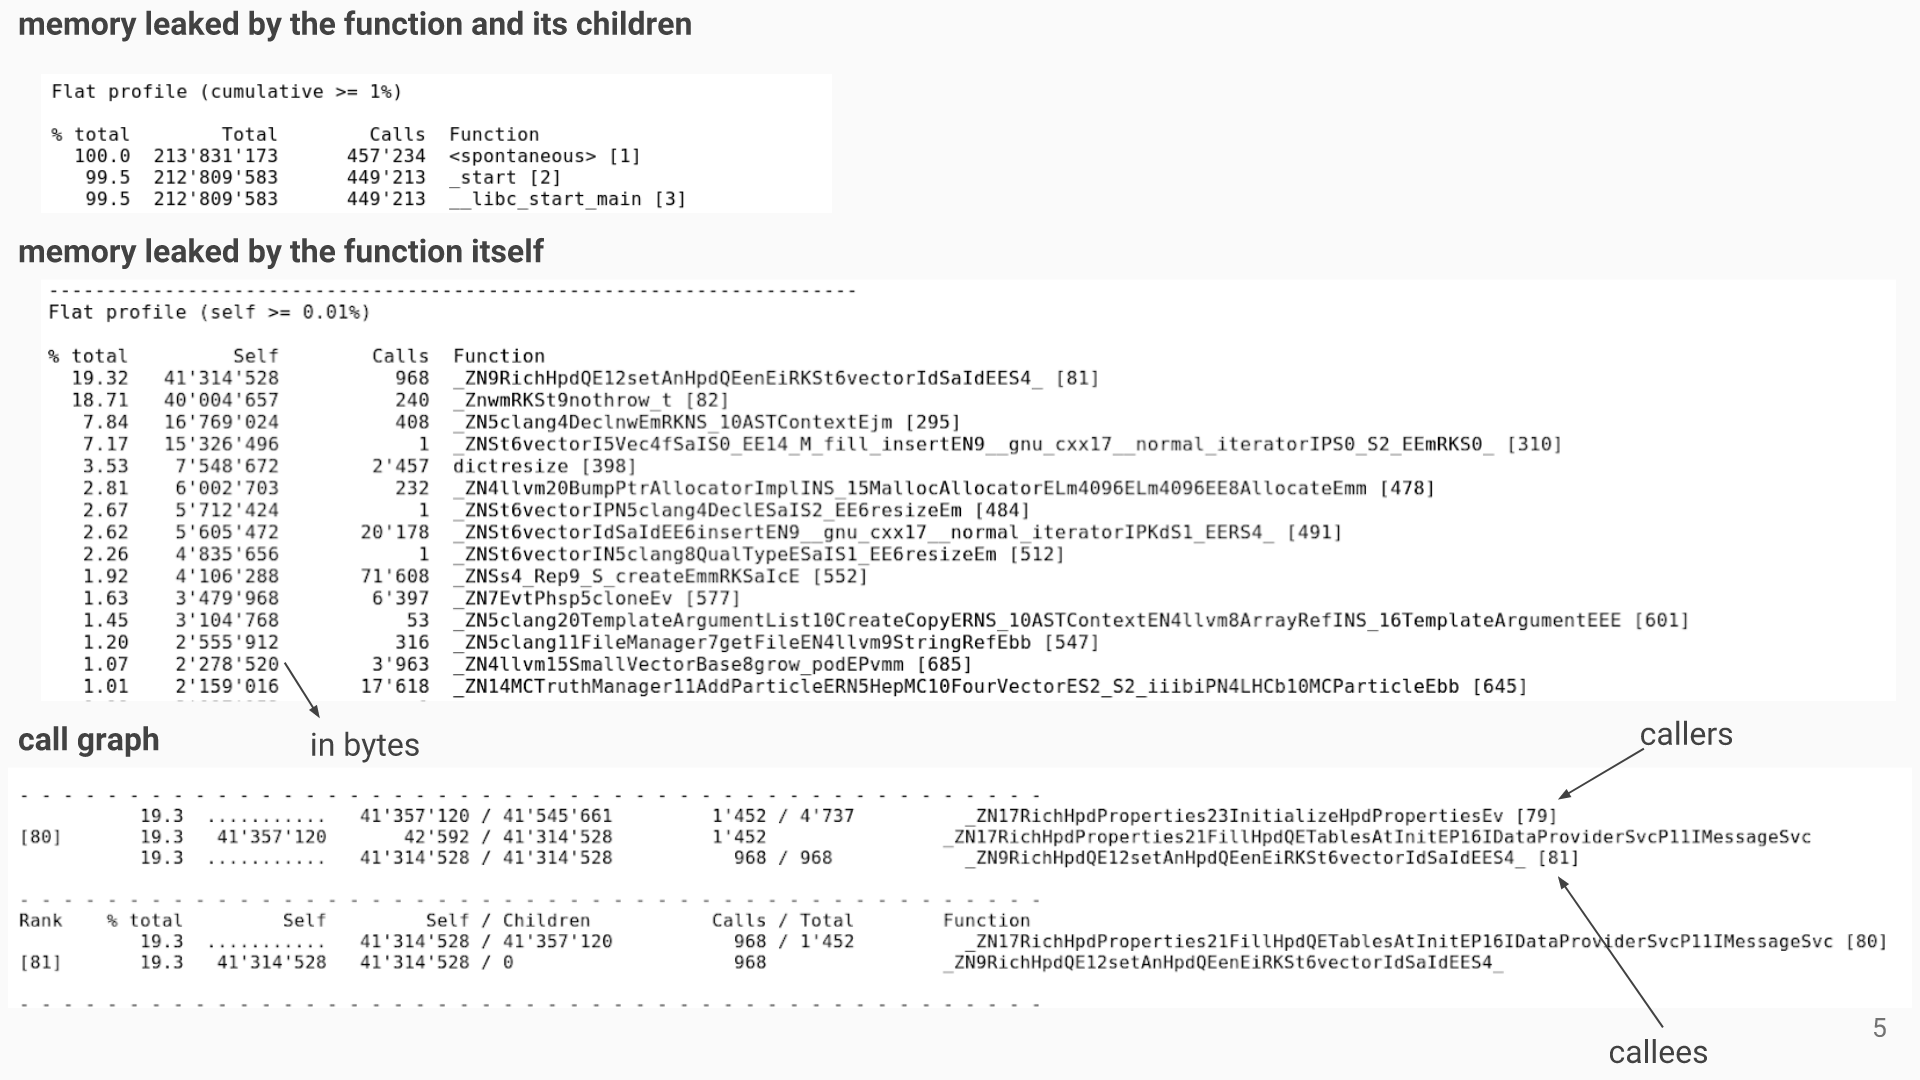
\includegraphics[width=1.09\textwidth]{igprof.png}
\end{frame}

\begin{frame}
\frametitle{\centerline{Big data tools for LHCbPR}}
\begin{itemize}
\setlength\itemsep{10pt}
\footnotesize
\item Data from tests pushed to Hadoop Distributed File System
\item Possibility to use Spark connector in SWAN notebooks to read those data
\item {\bf Interactive} exploration, {\bf collaboration} on tests reports
\item Needs to belong to the \texttt{ai-hadoop-users} e-group
% \item<1-> How can we profit from the {\bf state-of-art technologies} like Hadoop?
% \item<1-> Increasing {\bf data volume} in LHCbPR
% \item<1-> {\bf Interactive} exploration, {\bf collaboration} on tests reports
\visible<1->{
\begin{tikzpicture}[
    %show background grid,
    >=stealth,
    node distance=1.7cm,
    database/.style={
      cylinder,
      cylinder uses custom fill,
      cylinder body fill=blue!20,
      cylinder end fill=blue!20,
      shape border rotate=90,
      aspect=0.25,
      minimum height=1.7em,
      draw
    }
  ]
    \node [block] (LHCbPR) at (0,0) {LHCbPR};
    \node [database, below of=LHCbPR] (mysql) {MySQL DBoD};
    \node [cloud, below of=mysql] (LHCbPR2FE) {LHCbPR2FE};
    \node [database] (eos) at (4,0) {EOS};
    \node [block, fill=yellow!20, text width=3em] (parquet) at (4,-1.5) {\tiny batch ingestion in Parquet format};
    \node [database] (hdfs) at (4,-3.5) {HDFS};
    \node [block, fill=yellow!20, text width=3em] (spark) at (6.5,-1.5) {Apache Spark};
    \node [cloud] (swan) at (10,0) {SWAN};
    \node [cloud, below of=swan] (zeppelin) {Apache Zeppelin};
    \node [cloud, below of=zeppelin] (jupyter) {Jupyter};
    \node [draw,rounded corners=2mm, fill=brown!30] at (0,-3.8) {\tiny currently in production};

    \draw[->,blue!50, line width=0.4mm] (LHCbPR) --  node[black,midway,above,font=\tiny]{} node[black,midway,below,font=\tiny]{} (mysql);
    \draw[->,blue!50, line width=0.4mm] (mysql) --  node[black,midway,right,font=\tiny]{} (LHCbPR2FE);
    \draw[->,blue!50, line width=0.4mm] (eos) -- (parquet);
    \draw[->,blue!50, line width=0.4mm] (parquet) -- (hdfs);
    \draw [->,blue!50, line width=0.4mm] (LHCbPR) -- node[black,midway,below,font=\tiny]{} (eos);
    \draw [->,blue!50, line width=0.4mm] (eos) -- (spark);
    \draw [->,blue!50, line width=0.4mm] (hdfs) -- (spark);
    \draw [->,blue!50, line width=0.4mm] (spark) -- (swan);
    \draw [->,blue!50, line width=0.4mm] (spark) -- (zeppelin);
    \draw [->,blue!50, line width=0.4mm] (spark) -- (jupyter);

    %% \path [->,blue!50] (mysql) -- (LHCbPR2FE);

    %% \draw[->,blue!50] (db1) -- ++(0,1) -- ($(db2)+(0,1)$) node[black,midway,above,font=\scriptsize]{merged, daily} node[black, midway,below,font=\scriptsize]{partitioned in Apache Parquet} -- (db2) ;

    \begin{pgfonlayer}{background}
    \node[surround] (background) [fit = (LHCbPR) (mysql) (LHCbPR2FE)] {};
    \end{pgfonlayer}

  \end{tikzpicture}
}

\end{itemize}
\end{frame}

\begin{frame}
\frametitle{SWAN notebooks for the analysis of tests results}
\begin{center}
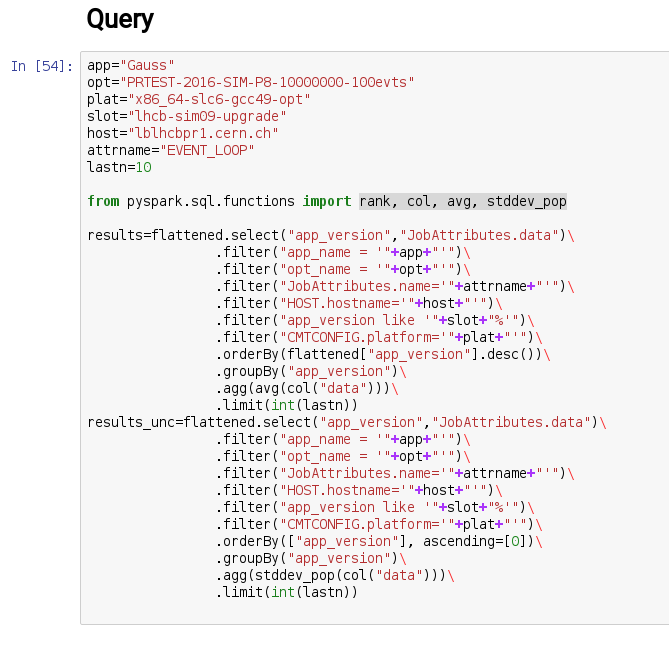
\includegraphics[width=0.53\textwidth]{query.png}
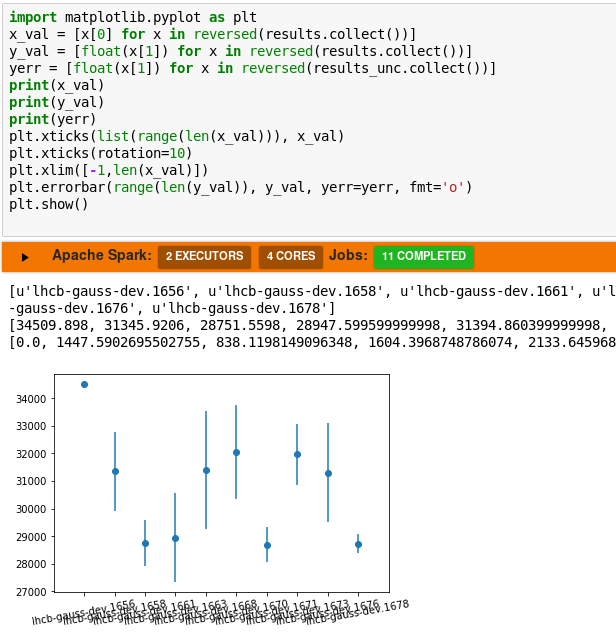
\includegraphics[width=0.47\textwidth]{notebook.png}

\end{center}
\end{frame}


\begin{frame}
\center Thank you! \\ Please give feedback on our \href{https://mattermost.web.cern.ch/lhcb/channels/lhcbpr2}{\beamergotobutton{mattermost channel}}

\end{frame}

%%%%%%%%%%%%%%%%%%%%%%%%%%%%%%%%%%%%%%%%%%%%%%%%%%%%%%%%%%%%%%%%%%%%%%%%%%%%%%%%%%%%%%%%%%%%%

%%%%%%%%%%%%%%%%%%%%%%%%%%%%%%%%%%%%%%%%%%%%%%%%%%%%%%%%%%%%%%%%%%%%%%%%%%%%%%%%%%%%%%%%%%%%%

%%%%%%%%%%%%%%%%%%%%%%%%%%%%%%%%%%%%%%%%%%%%%%%%%%%%%%%%%%%%%%%%%%%%%%%%%%%%%%%%%%%%%%%%%%%%%
%%%%%%%%%%%%%%%%%%%%%%%%%%%%%%%%%%%%%%%%%%%%%%%%%%%%%%%%%%%%%%%%%%%%%%%%%%%%%%%%%%%%%%%%%%%%%
%%%%%%%%%%%%%%%%%%%%%%%%%%%%%%%%%%%%%%%%%%%%%%%%%%%%%%%%%%%%%%%%%%%%%%%%%%%%%%%%%%%%%%%%%%%%%
\backupbegin
% And your backup slides here
%% \appendix

\begin{frame}
\frametitle{\centerline{LHCbPR - Resources}}
\begin{itemize}
\footnotesize
\item<1-> Web application:

\url{https://lblhcbpr.cern.ch}

\url{https://lblhcbpr.cern.ch/api/}

\url{https://gitlab.cern.ch/lhcb-core/LHCbPR2FE}
\item<1-> API service:

\url{https://gitlab.cern.ch/lhcb-core/LHCbPR2BE}
\item<1-> ROOT HTTP service:

\url{https://gitlab.cern.ch/lhcb-core/LHCbPR2ROOT}
\item<1-> Tests’ output handlers:

\url{https://gitlab.cern.ch/lhcb-core/LHCbPR2HD}
\item<1-> Project builder:

\url{https://gitlab.cern.ch/lhcb-core/LHCbPR2}
\item<1-> Jenkins configuration

\url{https://gitlab.cern.ch/lhcb-core/LbNightlyTools}
\item<1-> Configuration of the periodic tests

\url{https://gitlab.cern.ch/lhcb-core/LHCbNightlyConf/}
\end{itemize}
\end{frame}

%% %% \begin{frame}
%% %% \frametitle{\centerline{Upgrade of simulation framework}}
%% %% \begin{itemize}
%% %% \footnotesize
%% %% \item<1-> {\bf Monte Carlo simulations} of high-energy collisions require {\bf significant computing resources}
%% %% \item<2-> Increase of needed resources after the upgrade {\bf cannot be compensated solely by technological advancements}
%% %% \item<3-> Analysis of the feasible ways of the {\bf speed improvements} of the simulation software
%% %% \item<4-> Evaluation of the {\bf optimal selections} to obtain an improved computing performance with satisfactory physics modelling
%% %% \item<5-> Moving the simulation application to a {\bf multi-core architecture}
%% %% \item<6-> Integration of the Gaudi framework with the multithreaded version of external tools like Geant4
%% %% \end{itemize}
%% %% \end{frame}

\backupend
